\documentclass[12pt]{article}

\usepackage{sbc-template}
\usepackage{graphicx}
\usepackage[utf8]{inputenc}
\usepackage[T1]{fontenc}
\usepackage{hyperref}
\usepackage{amsmath}
\usepackage{booktabs}
\usepackage{multirow}
\usepackage{float}
\usepackage{subcaption}
\usepackage{xcolor}
\usepackage[authoryear,round]{natbib}

\sloppy

\title{How Well Do Small Language Models Understand the Brazilian Educational Context? An Evaluation on ENEM, FUVEST and Unicamp}

% Correção aplicada: Quebra de linha manual com \\ para evitar o corte na margem
\author{Anonymous Authors}

\address{Anonymous Institution
  \email{anonymous}
}

\begin{document}

\maketitle

\begin{abstract}
We present a benchmark for Small Language Models (SLMs) on Brazilian high-stakes exams, a setting combining Portuguese reasoning, educational knowledge, and image-based questions rarely covered in prior work. Unlike earlier benchmarks centered on English or native multimodal models, we replace visual items with rich textual descriptions to enable a unified zero-shot evaluation of 12 models on multidisciplinary questions. Our results show that compact models are much cheaper than larger LLMs, but their performance remains uneven across subjects and visual-context demands. These findings highlight both the promise and the current limits of SLMs for scalable educational evaluation in Brazilian Portuguese.

\vspace{6pt}
\noindent \textbf{Keywords:} Small Language Models, Educational Context, Zero-shot Evaluation, Portuguese, LLM Evaluation.
\end{abstract}

\section{Introduction}
\label{sec:intro}
Recent advances in small language models (SLMs) have made compact deployment a realistic option where latency, memory, and inference costs are critical, though their performance on localized educational tasks remains less explored than that of larger systems \cite{nguyen2025survey,pham2025slmbench}. While general evaluation frameworks advocate for protocols reflecting practical deployment constraints rather than accuracy alone \cite{liang2023helm}, testing these models within culturally and linguistically grounded domains provides essential insights into their real-world utility.

To address this, we evaluate compact and reference models on 3,710 Portuguese questions from Brazil's most prominent high-stakes examinations: ENEM, the national secondary-school exam managed by INEP to assess basic education and higher education access \cite{inep_enem}, alongside FUVEST and Unicamp, the highly selective admissions pathways for USP \cite{usp_fuvest} and Unicamp \cite{comvest_unicamp}, respectively. To isolate textual reasoning, image-dependent items are converted into rich textual descriptions \cite{das2024examsv}, and models are queried in a zero-shot setting under strict JSON output constraints \cite{lu2025learning}. This setup measures how modern compact architectures handle localized educational content while benchmarking the cost-performance frontier and the limits of structured zero-shot reasoning.

In summary, our main contributions are: (1) a comprehensive evaluation of modern SLMs on major Brazilian university entrance exams; (2) a granular analysis of model performance mapped across specific disciplines and cognitive capabilities; (3) an empirical assessment of the performance penalty incurred by replacing visual questions with textual descriptions; and (4) a detailed cost-benefit analysis delineating the Pareto frontier for deploying SLMs in resource-constrained educational environments.

\section{Related Work}
\label{sec:related}
Research on small language models has converged on the idea that compactness can be achieved without abandoning utility, but that performance must be interpreted together with resource use. Nguyen et al. \cite{nguyen2025survey} provide a recent survey of SLM architectures and training strategies, while Pham et al.'s SLM-Bench \cite{pham2025slmbench} explicitly evaluates trade-offs across correctness, computation, and energy consumption under controlled hardware conditions. Together, these works motivate evaluating compact models not only by answer accuracy but also by their practical deployment cost.

A second relevant line of work studies language models on Brazilian and Portuguese educational benchmarks. BLUEX \cite{almeida2023bluex} established one of the first large Brazilian exam benchmarks with image annotations and capability metadata, making it useful for reasoning-oriented evaluation in Portuguese. Nunes et al. \cite{nunes2023evaluating} then showed that ENEM can be used to probe general reasoning in Brazilian Portuguese, and Locatelli et al. \cite{locatelli2024examining} extended this direction by comparing model and human answer distributions on standardized national exams. More recently, Sabiá and Sabiá-2 \cite{pires2023sabia,almeida2024sabia} and Alvorada-Bench \cite{godoy2025alvorada} reinforced the idea that exam-style evaluation in Portuguese is a meaningful test bed for local-language models, with Alvorada-Bench especially emphasizing that Brazilian exams can support large-scale, text-only reasoning evaluation.

\section{Methods}
\label{sec:methods}

Our evaluation pipeline is designed to systematically assess the textual reasoning and instruction-following capabilities of Small Language Models (SLMs) within the context of the Brazilian educational system. We rely on a dataset comprising questions from ENEM, FUVEST (USP), and Unicamp, replace visual assets with text descriptions to isolate reasoning, and use a zero-shot prompting protocol to elicit strict JSON responses.

\subsection{Dataset Configuration and Adaptation}
The initial dataset comprises 3,710 multidisciplinary questions (Portuguese, Mathematics, History, Physics, etc.) in their original Portuguese formulation, testing logic, culture-specific knowledge, and text comprehension. To enable automated evaluation, we restricted the benchmark to multiple-choice items containing a single discrete target answer, retaining the original statements, alternatives, official templates, and metadata (year and subject). Only questions with valid answer notes were used. After filtering out nine items with unrecoverable visual artifacts, the final evaluation set yielded 3,701 questions, spanning 2009--2023 for ENEM (2,595 items), and 2018--2024 for FUVEST (626 items) and Unicamp (480 items).

To isolate textual reasoning capabilities consistently across all sub-14B models, questions containing visual components (graphs, diagrams, maps) were programmatically adapted by substituting visual assets with rich, offline-generated text descriptions. Rather than relying on subjective manual assessment, the choice of the Vision-Language Model (VLM) descriptor was driven by an empirical downstream accuracy optimization sweep across an evaluation fleet. Tested architectures included Llama-3.2-11B-Vision-Instruct, Qwen-VL (30B, 235B), ByteDance Seed-1.8 and Seed-2.0-mini, Gemma-3 (4B, 12B, 27B), Llama-4 variants (Maverick-17B, Scout-17B), Mistral-Small-3.2-24B, NVIDIA-Nemotron-Nano-12B-v2-VL, and GLM-4.6V. ByteDance Seed-1.8 yielded the highest downstream accuracy and was selected as the pipeline's descriptor, serving as a pipeline-level optimization rather than an absolute baseline for visual-description quality.

\subsection{Model Fleet Selection}
To map the baseline reasoning limits, we composed a fleet of 12 distinct models. Our focus is a core subset of SLMs with $\le$ 14B parameters, contrasting their accuracy against significantly larger reference models.
The primary evaluated SLMs include:
\begin{itemize}
    \item \textbf{Gemma Family:} Gemma-3-4B-IT and Gemma-3-12B-IT;
    \item \textbf{Llama Family:} Meta-Llama-3.1-8B-Instruct;
    \item \textbf{Qwen Family:} Qwen3.5-0.8B, Qwen3.5-2B, and Qwen3.5-4B.
\end{itemize}

In order to define capability bounds and Pareto frontiers for reasoning, six additional reference Large Language Models (LLMs) were assessed, comprising Gemma-3-27B-IT, Gemma-4-31B-IT, Llama-3.3-70B-Instruct-Turbo, DeepSeek-V4-Flash, DeepSeek-V3.2, and GLM-5.1.

\subsection{Evaluation Protocol and Prompting Strategy}
Deploying these models in an API environment requires enforcing strict structural compliance. We employ a zero-shot prompting strategy crafted to enforce output determinism. The system prompt instructs each model to act as a university entrance exam expert and to emit only a single JSON object, without Markdown blocks or conversational text.

The JSON schema mandates two components: \texttt{reasoning\_summary} (an explanation bounded to 150 words in Portuguese detailing the reasoning process) and \texttt{predicted\_answer} (the selected letter or value, constrained against the dynamically parsed allowed options for each unique question).

To address provider-level parsing volatility, we implemented a custom tolerant JSON response parser capable of recovering truncated responses or correcting minor deviations. Models were executed with deterministic parameters ($\text{temperature} = 0$).

\section{Results}
\label{sec:results}

We report the execution of the zero-shot reasoning pipeline across the 12 selected models. The results map baseline capabilities across datasets, explore the models' disciplinary competences, examine performance by modality and capability annotations, and evaluate chronological robustness.

\subsection{Overall Performance Across Datasets}
Our cross-dataset evaluation demonstrates a stark capability divide between sub-14B parameter Small Language Models (SLMs) and their larger counterparts.


Table~\ref{tab:accuracy} details the exact average accuracies across the benchmark subsets. Predictably, frontier models established the capability ceiling in our benchmark, with GLM-5.1 leading the overall average accuracy (92.04\%), followed closely by Gemma-4-31B-IT (90.43\%) and the DeepSeek-V4/V3.2 family $\sim$87--88\%. Notably, despite possessing a fraction of the parameters of the DeepSeek variants, Gemma-4-31B-IT surpassed them, highlighting exceptional architectural efficiency. These models exhibited robust domain transfer, performing consistently across ENEM's extensive contextual questions and the denser, more direct formats of FUVEST and Unicamp.

Inference costs were computed from provider pricing using observed token counts and normalized to USD per 1,000 questions (excluding offline VLM generation). Plotting operational costs against accuracy metrics delineates a clear SLM Pareto frontier across all datasets (Fig.~\ref{fig:cost_benefit_all}). 

While the smallest configurations (e.g., 0.8B) offer negligible utility due to low baseline accuracy, architectures in the 4B to 12B range (such as Gemma-3-12B-IT and Qwen3.5-4B) establish a highly aggressive cost-efficiency sweet spot. Although their absolute reasoning accuracy trails the largest reference models, their drastically lower operational overhead presents a highly viable architectural compromise for resource-constrained public educational deployments within emerging contexts like Brazil.

\begin{figure}[htbp]
  \centering
  \makebox[\textwidth][c]{%
    \begin{subfigure}{0.55\textwidth}
      \centering
      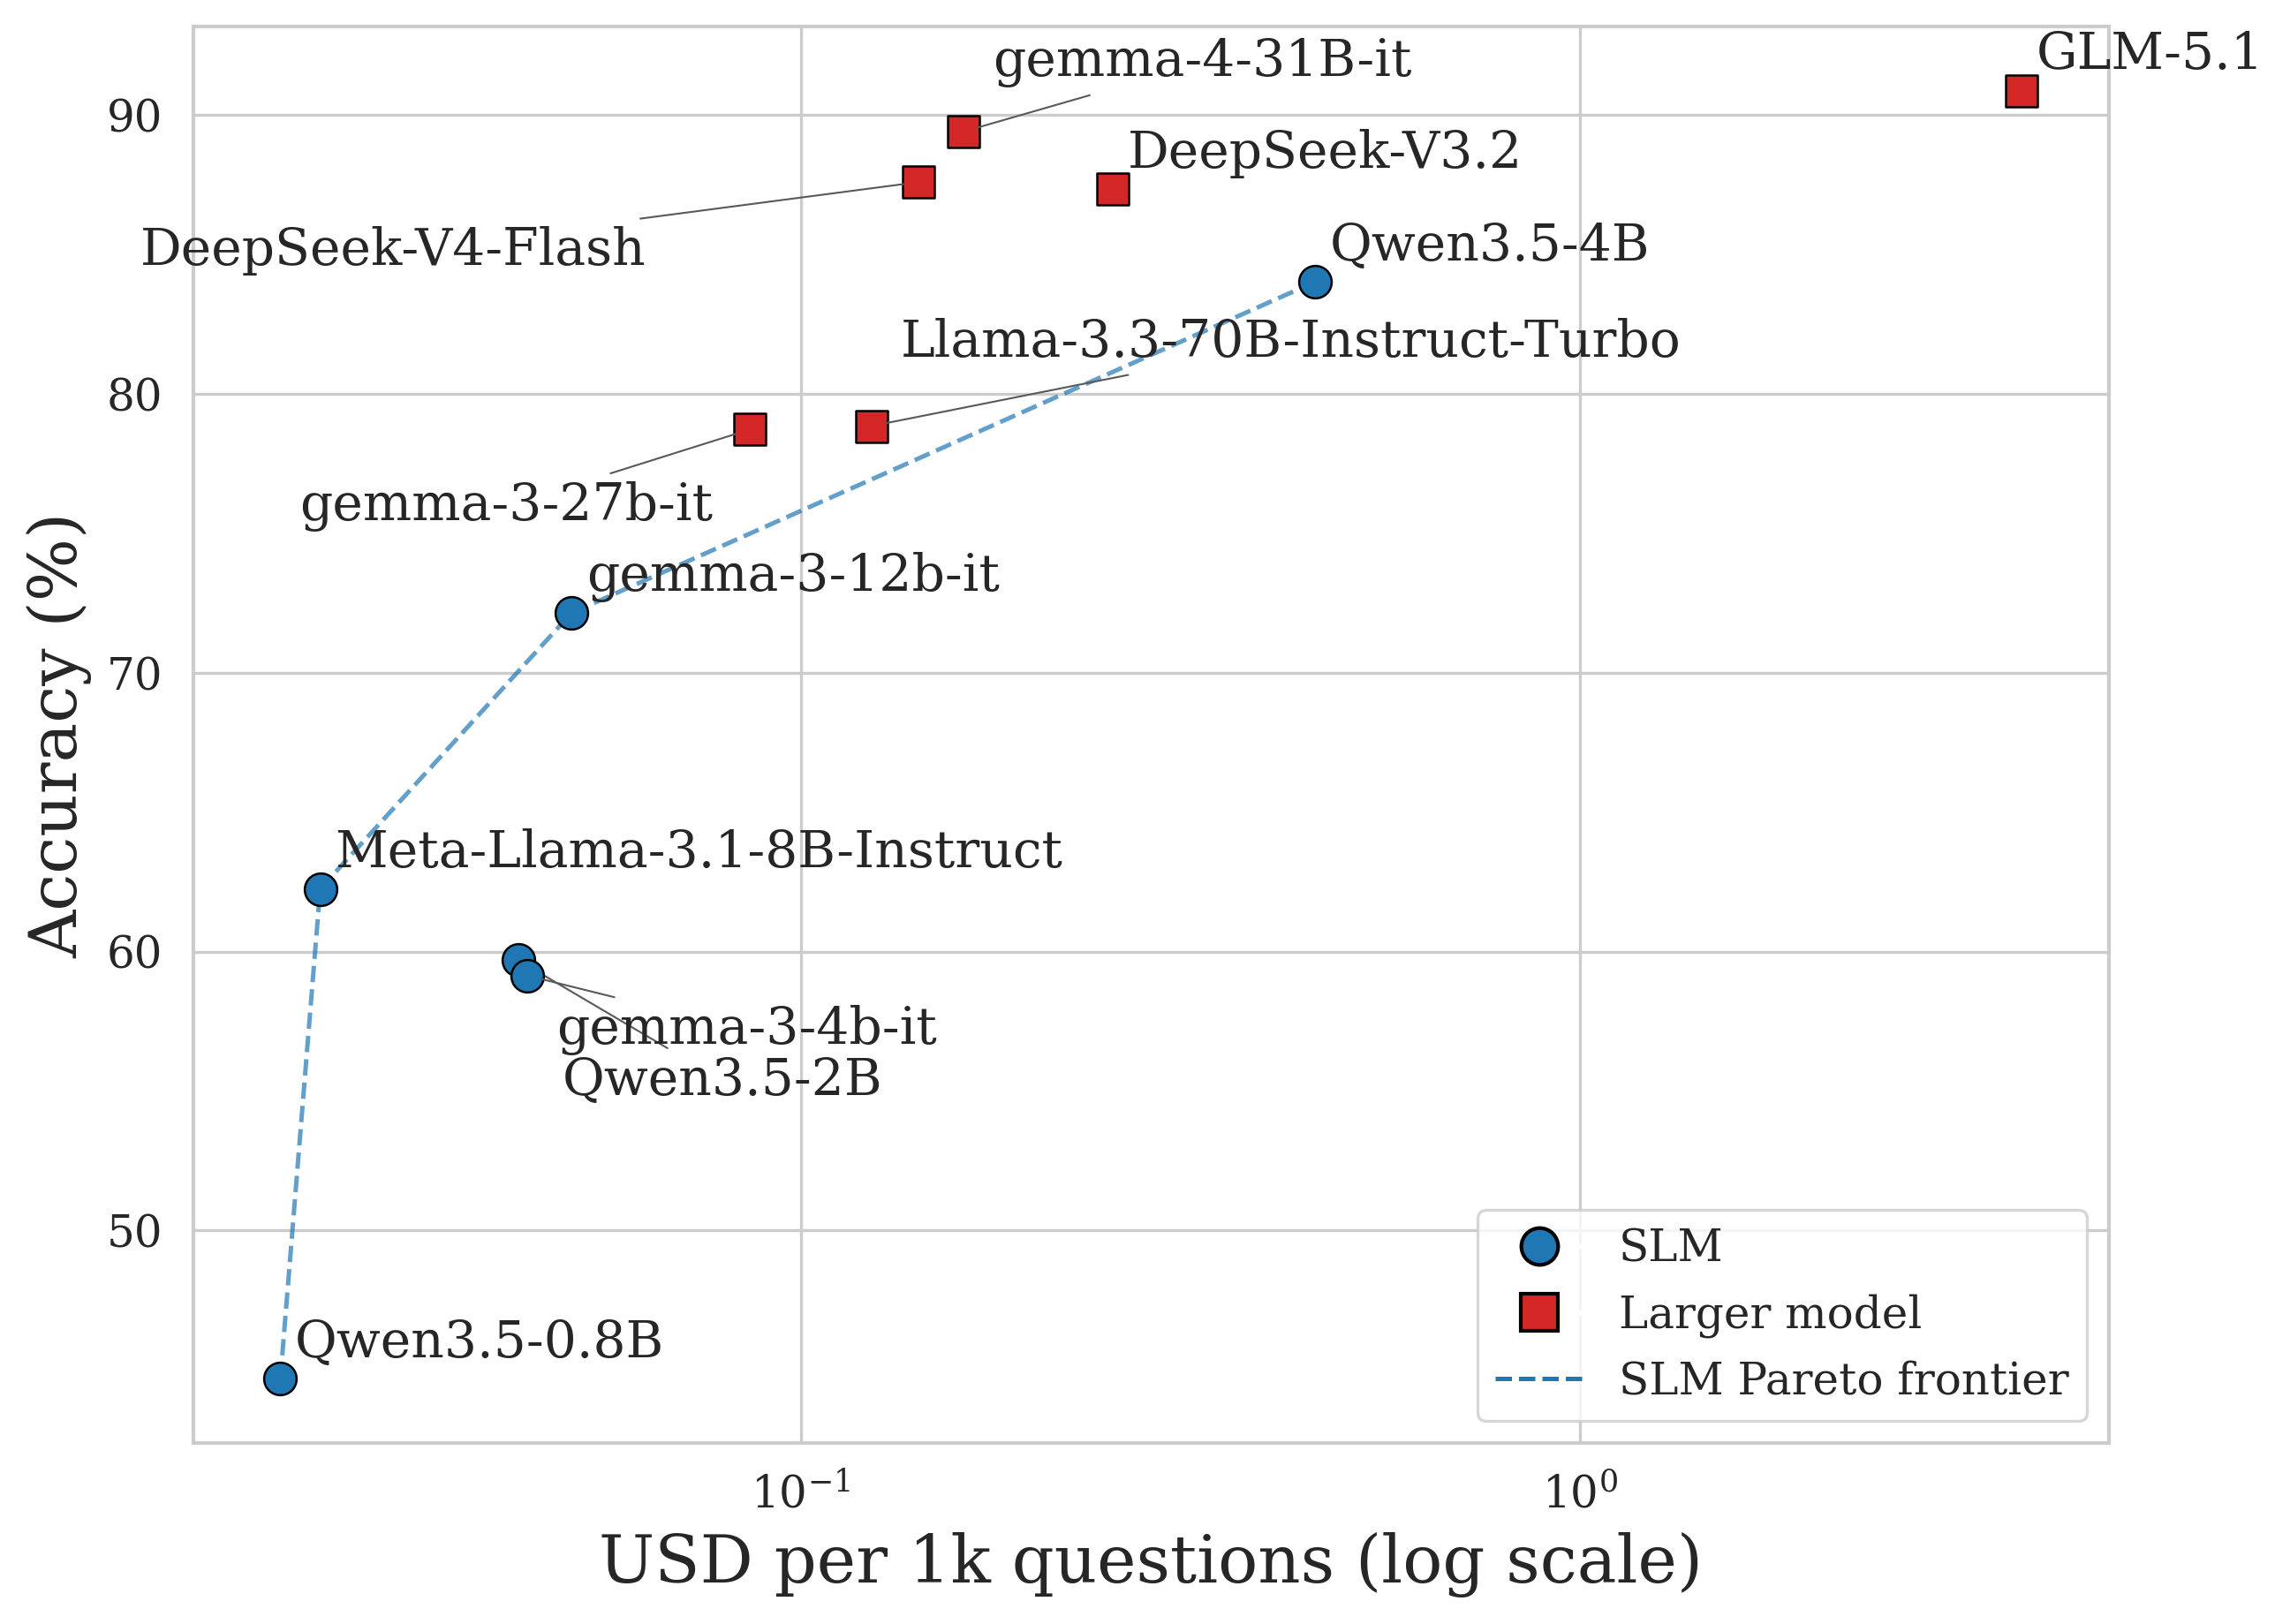
\includegraphics[width=\textwidth]{figures/cost_benefit_enem.png}
      \caption{ENEM}
    \end{subfigure}%
    \hspace{0.02\textwidth}
    \begin{subfigure}{0.55\textwidth}
      \centering
      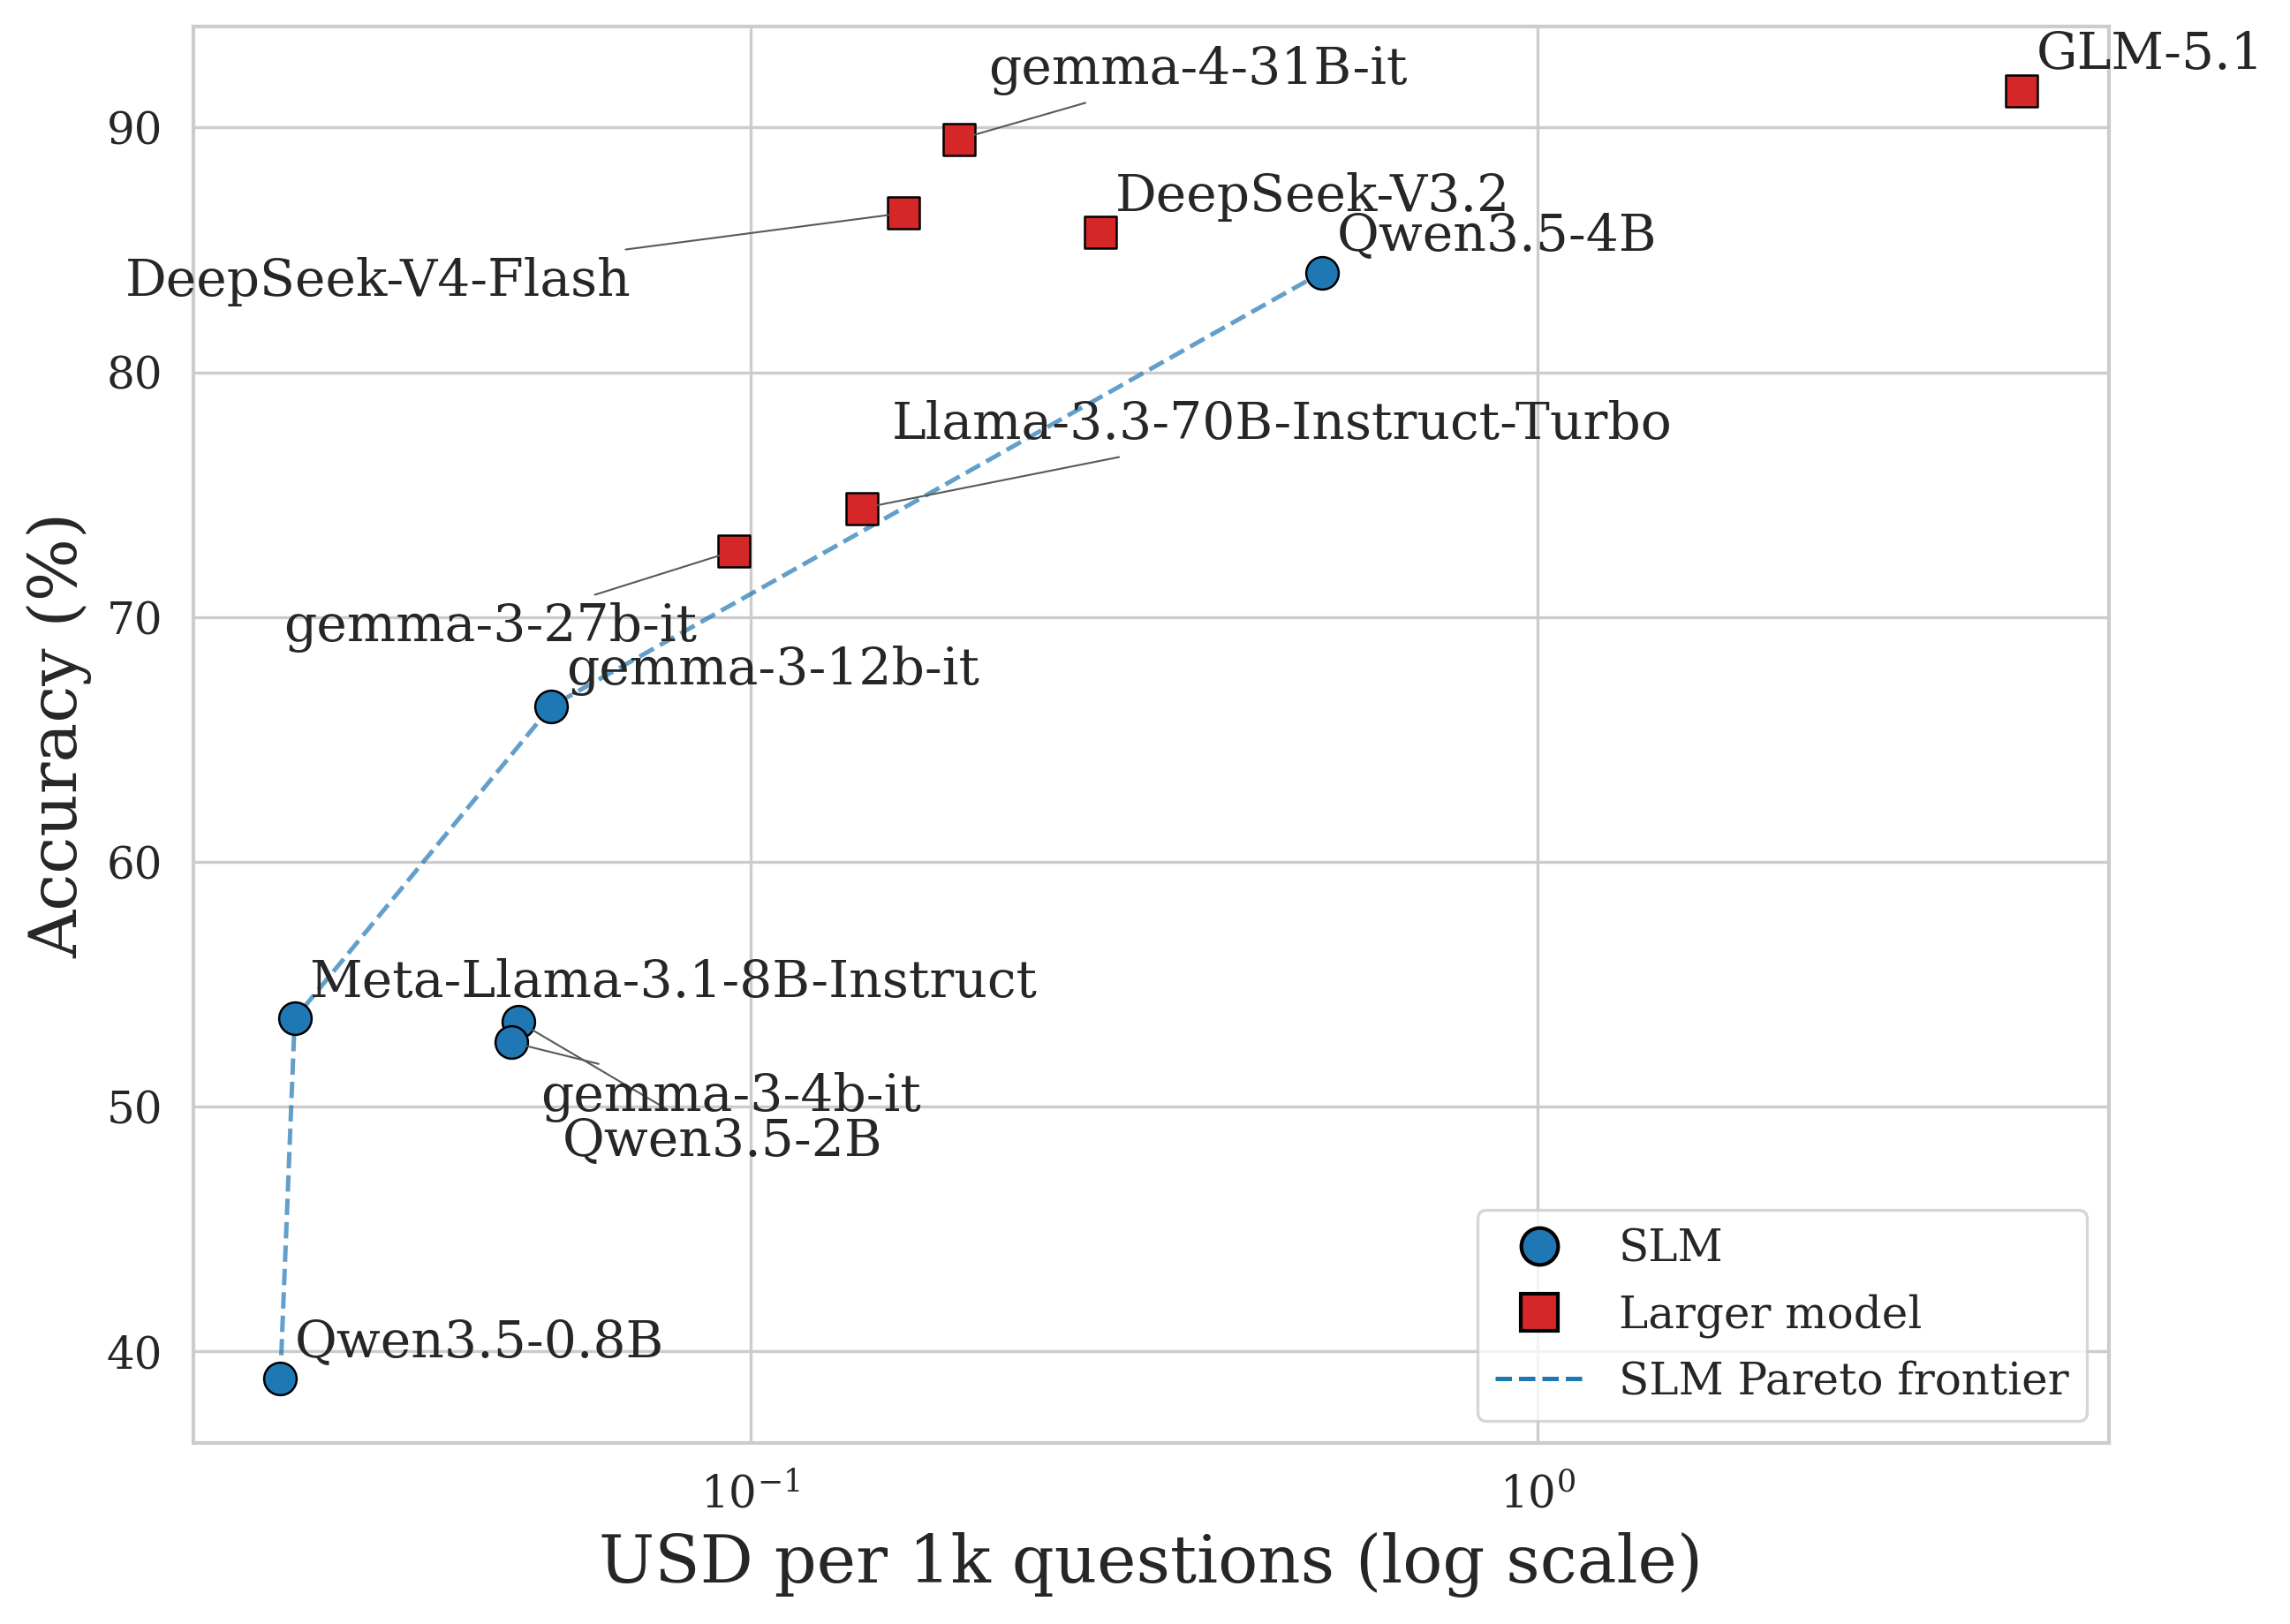
\includegraphics[width=\textwidth]{figures/cost_benefit_fuvest.png}
      \caption{FUVEST}
    \end{subfigure}%
  }

  \vspace{0.4cm}

  \begin{subfigure}{0.65\textwidth}
    \centering
    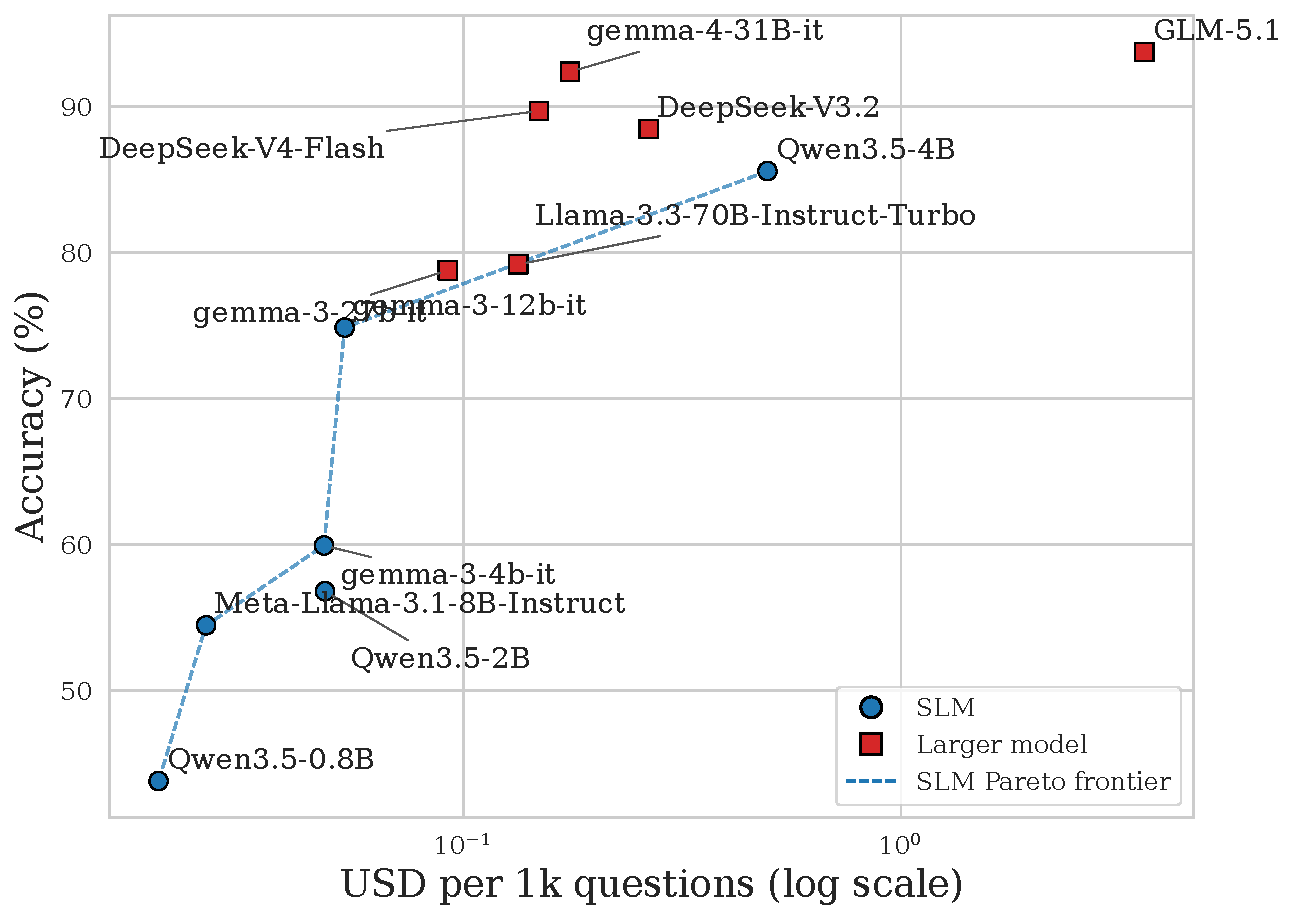
\includegraphics[width=\textwidth]{figures/cost_benefit_unicamp.pdf}
    \caption{Unicamp}
  \end{subfigure}
  \caption{Cost-benefit scatter plots mapping model accuracy against normalized USD cost per 1k queries across ENEM, FUVEST, and Unicamp datasets. The dashed lines denote the SLM Pareto frontiers.}
  \label{fig:cost_benefit_all}
\end{figure}

\begin{table}[htbp]
\caption{Cross-dataset average accuracy (\%) across the evaluated models, grouped by model class (LLM references vs. SLMs).}
\label{tab:accuracy}
\centering
\begin{tabular*}{\textwidth}{@{\extracolsep{\fill}} l l r c c c c}
\toprule
\textbf{Class} & \textbf{Model} & \textbf{Params (B)} & \textbf{ENEM} & \textbf{FUVEST} & \textbf{Unicamp} & \textbf{Mean} \\
\midrule
\multirow{6}{*}{\textbf{LLM}} 
& GLM-5.1 & 754.0 & 90.87 & 91.51 & 93.74 & \textbf{92.04} \\
& Gemma-4-31B-IT & 31.0 & 89.40 & 89.52 & 92.37 & 90.43 \\
& DeepSeek-V4-Flash & 284.0 & 87.59 & 86.51 & 89.69 & 87.93 \\
& DeepSeek-V3.2 & 671.0 & 87.35 & 85.71 & 88.45 & 87.17 \\
& Llama-3.3-70B-Instruct & 70.0 & 78.84 & 74.44 & 79.18 & 77.49 \\
& Gemma-3-27B-IT & 27.0 & 78.72 & 72.70 & 78.76 & 76.73 \\
\midrule
\multirow{6}{*}{\textbf{SLM}}
& Qwen3.5-4B & 4.0 & 84.02 & 84.08 & 85.57 & \textbf{84.55} \\
& Gemma-3-12B-IT & 12.0 & 72.14 & 66.35 & 74.85 & 71.11 \\
& Gemma-3-4B-IT & 4.0 & 59.14 & 52.62 & 59.92 & 57.23 \\
& Meta-Llama-3.1-8B-Instruct & 8.0 & 62.25 & 53.59 & 54.45 & 56.76 \\
& Qwen3.5-2B & 2.0 & 59.69 & 53.46 & 56.78 & 56.65 \\
& Qwen3.5-0.8B & 0.8 & 44.68 & 38.87 & 43.78 & 42.44 \\
\bottomrule
\end{tabular*}

\vspace{6pt}
\parbox{\textwidth}{\footnotesize \noindent For MoE models, total and active parameter counts differ; DeepSeek-V4-Flash, for example, has 284B total parameters and 13B active parameters per token. Total Params (B) denotes the model scale in billions of parameters.}
\end{table}

In contrast, the SLM group presented a different behavior patern. The highest-performing compact models varied across subsets, with Qwen3.5-4B demonstrating notable resilience, reaching 84.5\% average accuracy and outperforming even larger references such as Gemma-3-27B. The Gemma-3-12B-IT model showed strong general proficiency (71\% average), clearly distancing itself from the smaller Gemma-3-4B-IT (57.2\%) and Llama-3.1-8B-Instruct (56.7\%). The smallest model, Qwen3.5-0.8B, struggled to maintain stable logical performance, scoring 42.44\% on average. Although this is clearly above random guessing for exams with five alternatives, it remains substantially below the other evaluated models and indicates limited reliability for autonomous educational reasoning.

\subsection{Performance by Discipline}
Breaking down accuracy by subject reveals substantial variation in SLM performance across the three exams, as aggregated in the granular breakdowns for ENEM, FUVEST, and Unicamp in Fig.~\ref{fig:heatmaps_disciplines}. These heatmaps suggest that language comprehension, linguistics, and humanities tend to be stronger domains for text-centric models across the benchmarks. Conversely, subjects heavily reliant on logic, mathematics, and physics pose significant hurdles regardless of the exam's source. These lower scores are consistent with known difficulties of smaller architectures in multi-step numeric deduction and formal reasoning, although a detailed qualitative error taxonomy remains outside our immediate investigative scope.

\begin{figure}[htbp]
  \centering
  \makebox[\textwidth][c]{%
    \begin{subfigure}{0.55\textwidth}
      \centering
      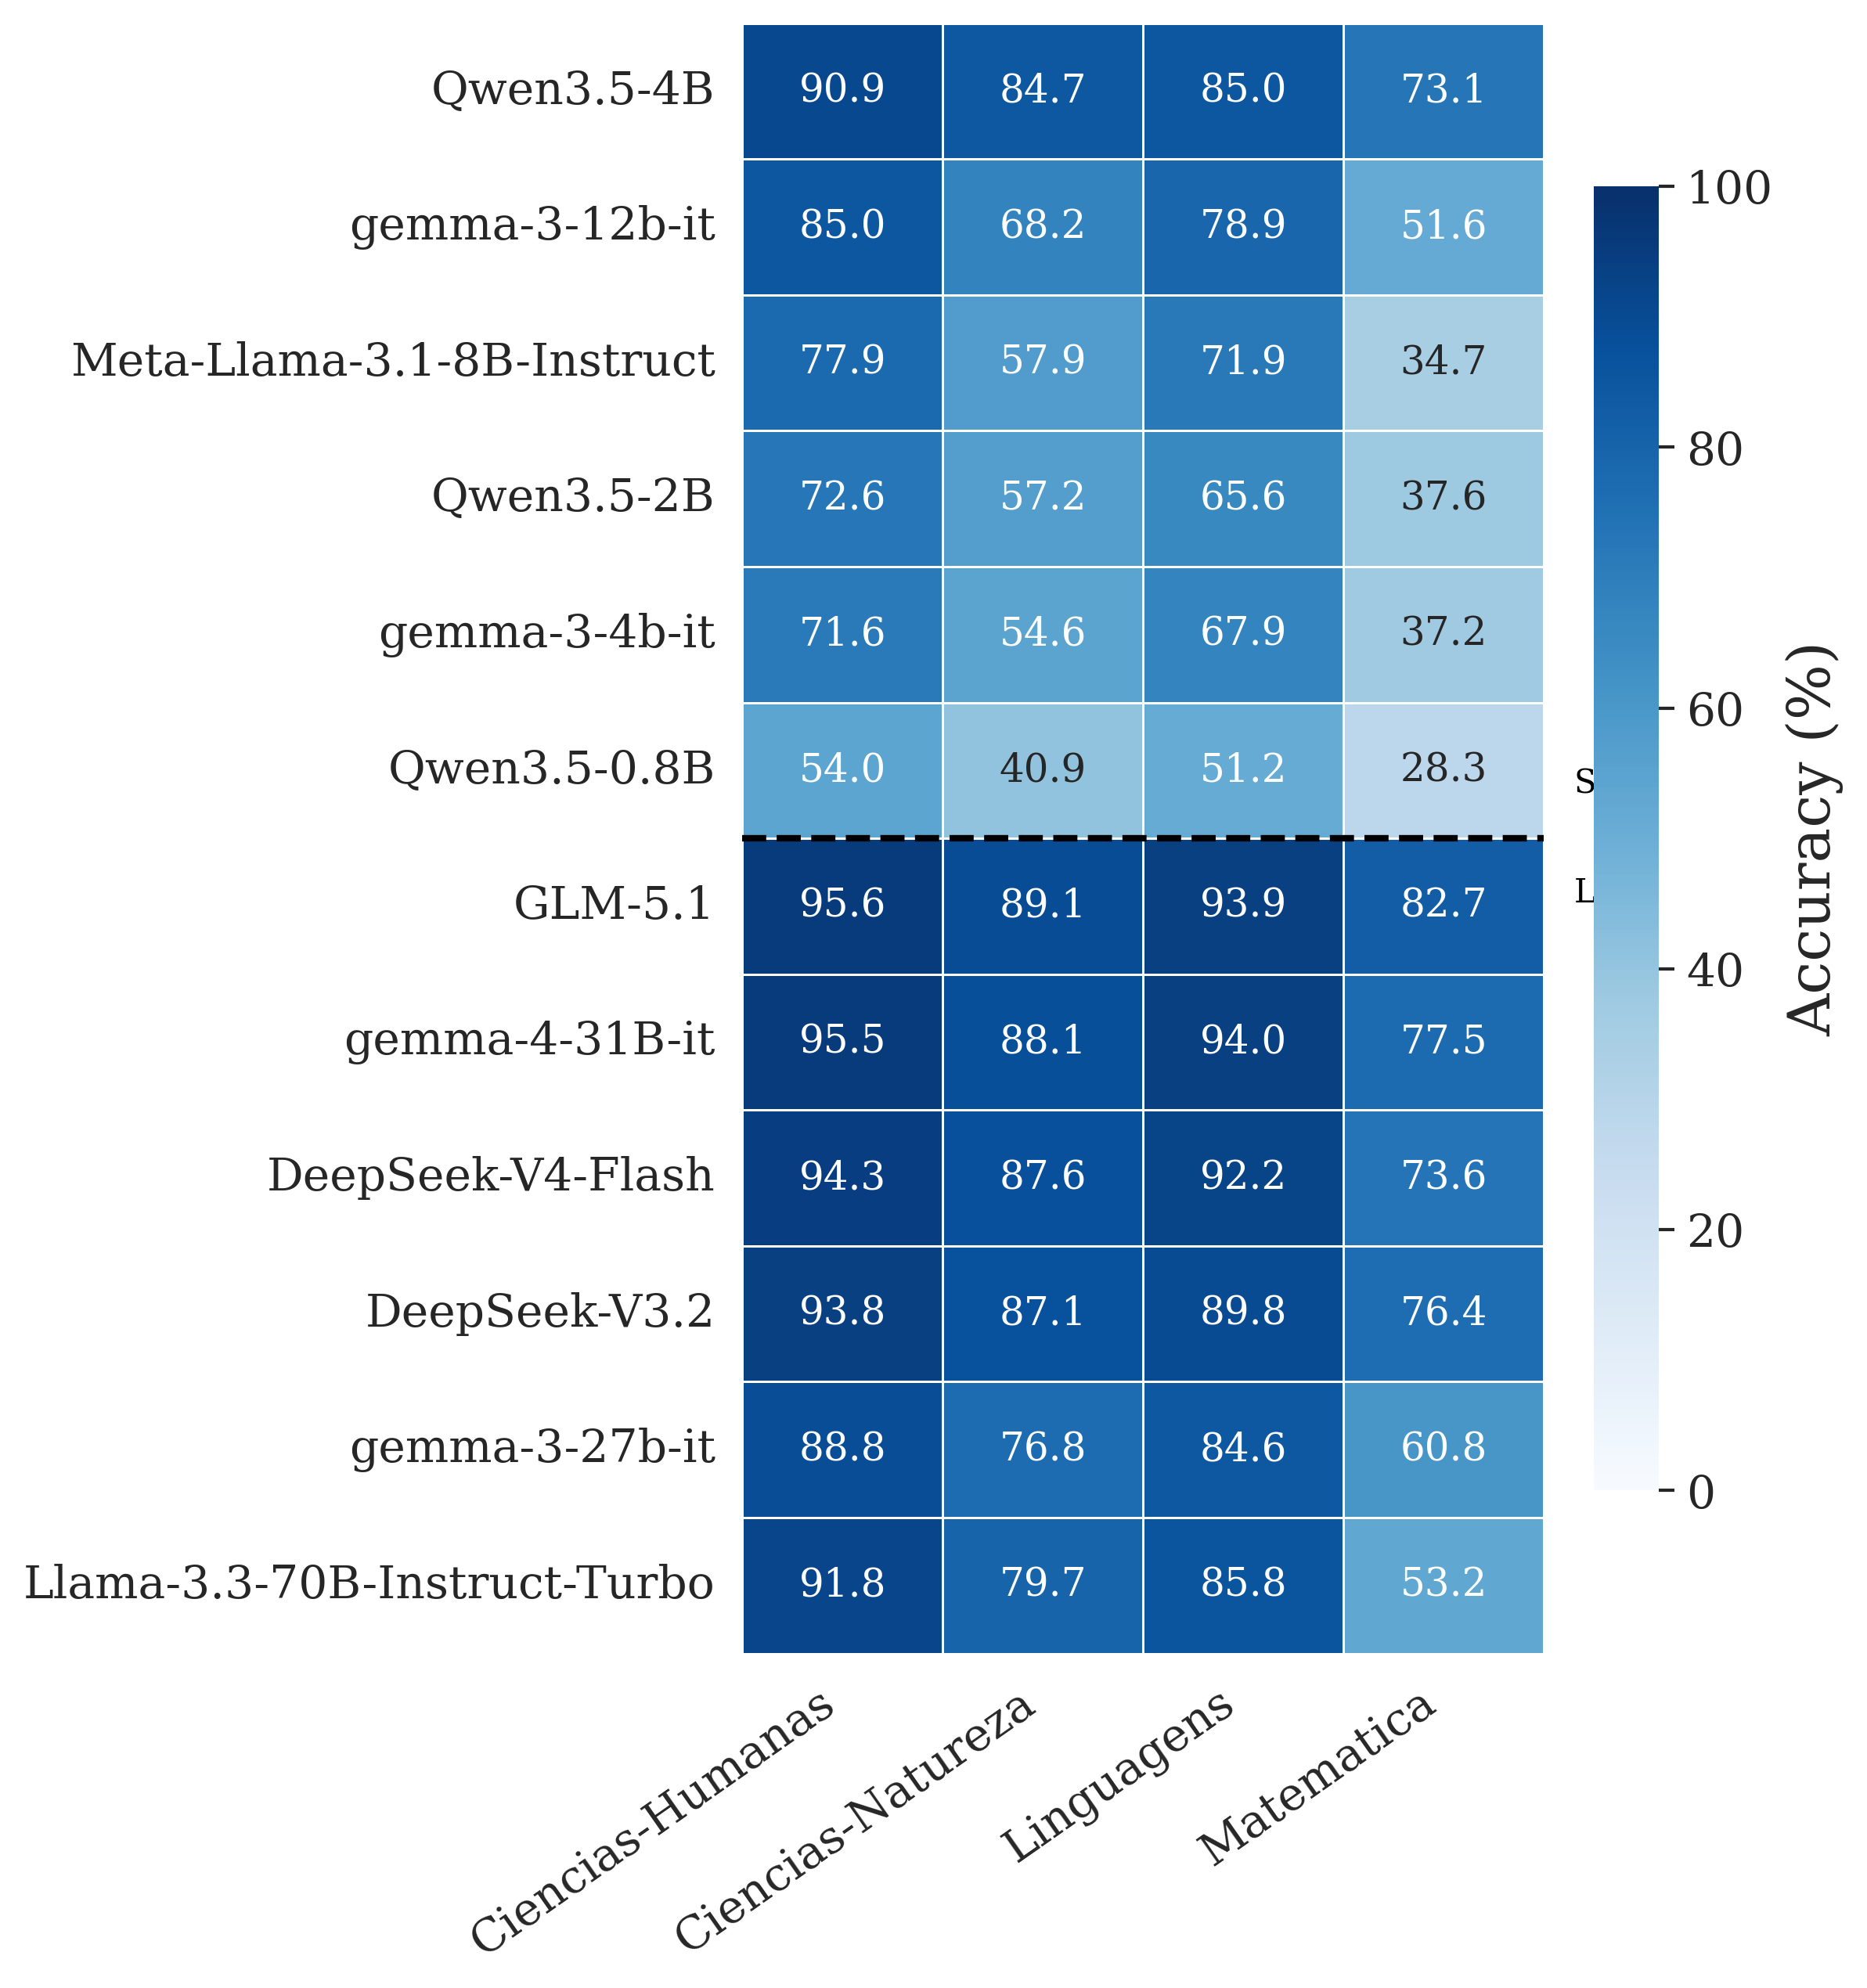
\includegraphics[width=\textwidth]{figures/subject_heatmap_enem.png}
      \caption{ENEM Subjects}
    \end{subfigure}%
    \hspace{0.02\textwidth}
    \begin{subfigure}{0.55\textwidth}
      \centering
      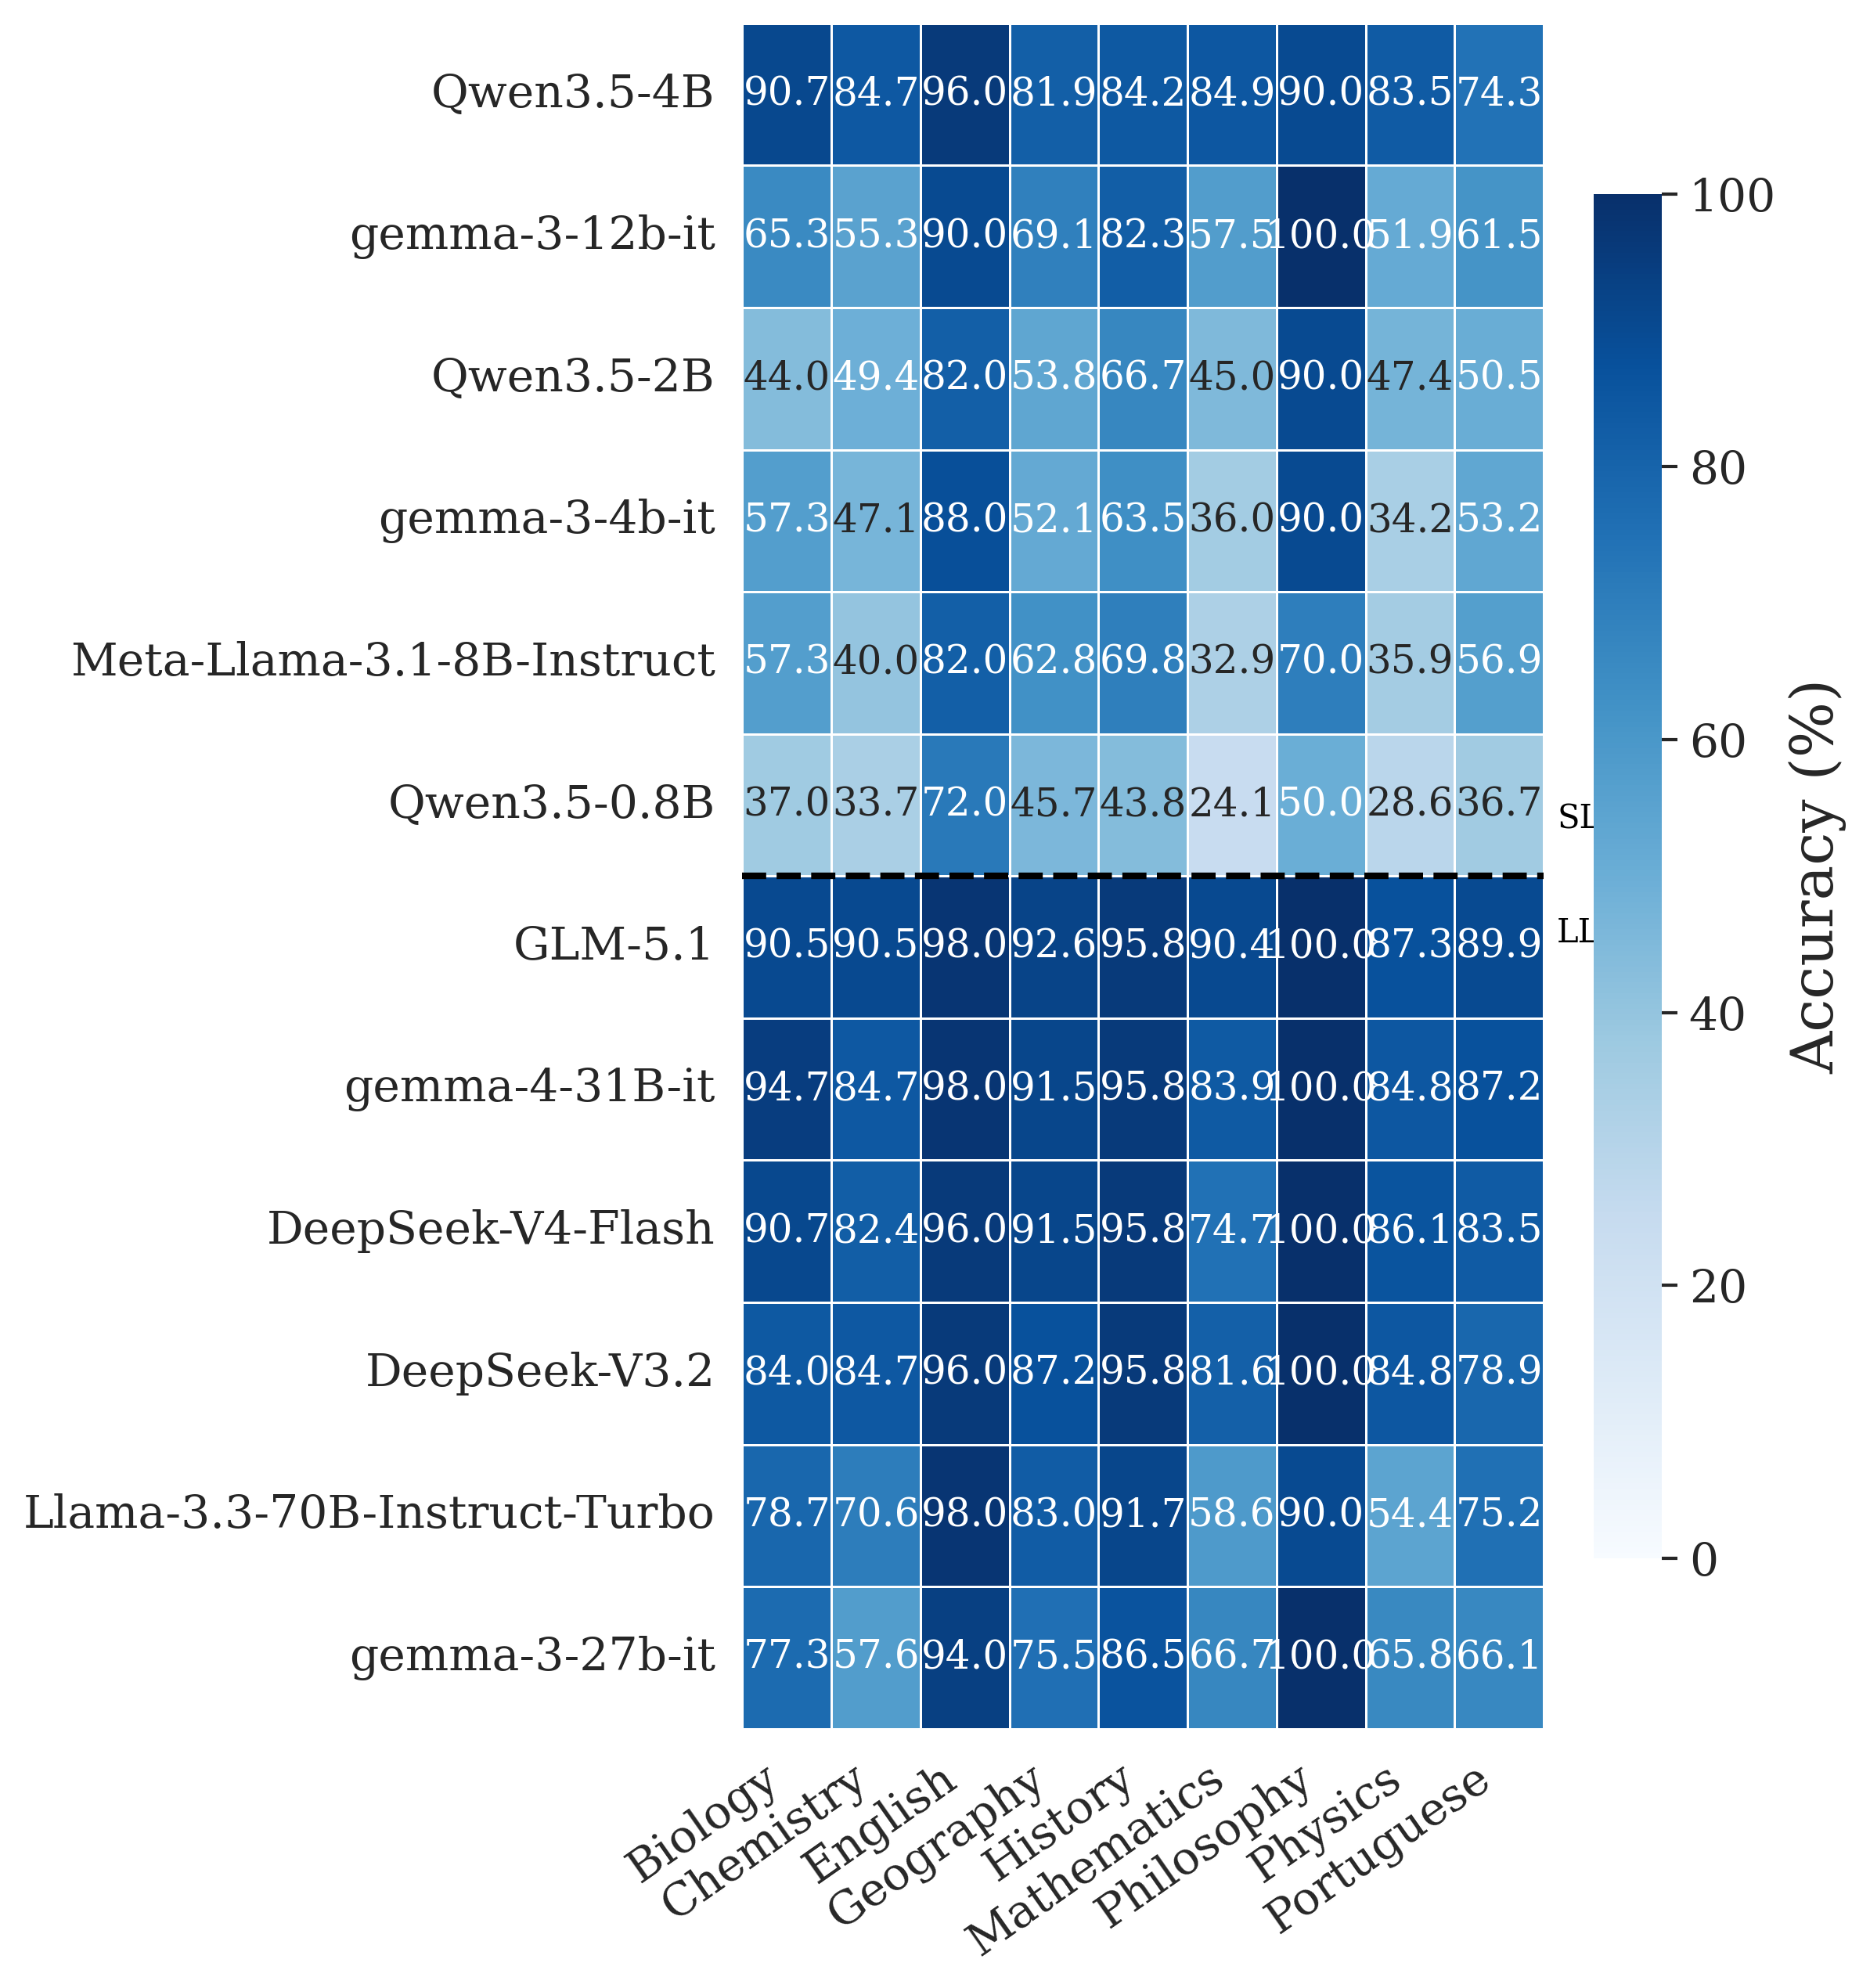
\includegraphics[width=\textwidth]{figures/subject_heatmap_fuvest.png}
      \caption{FUVEST Subjects}
    \end{subfigure}%
  }

  \vspace{0.4cm}

  \begin{subfigure}{0.65\textwidth}
    \centering
    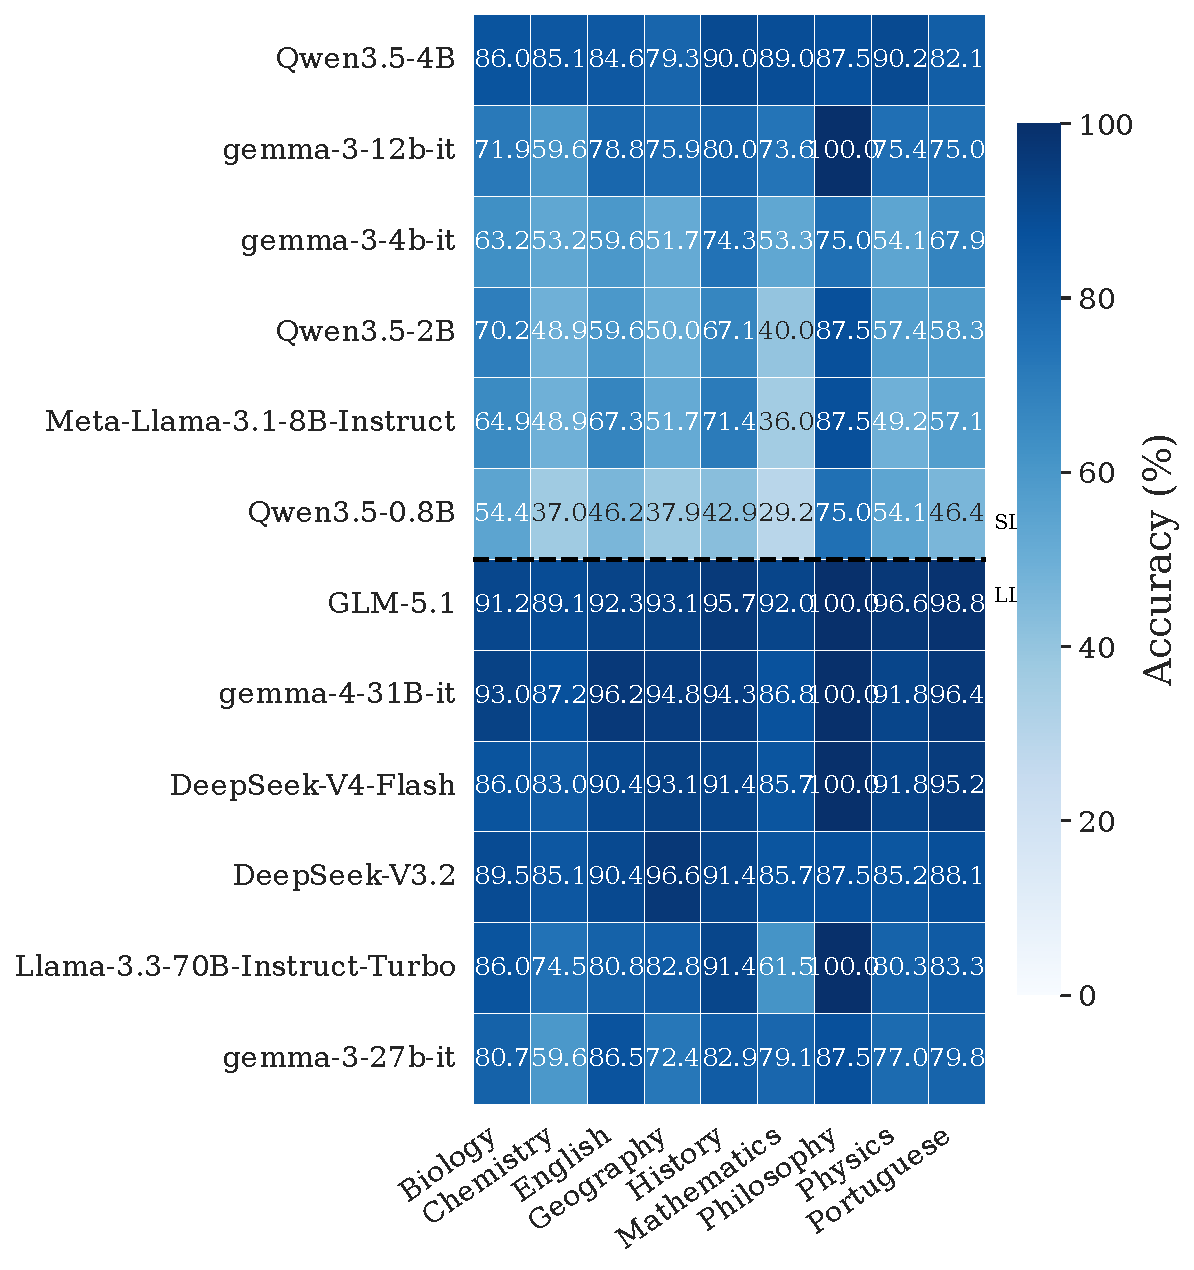
\includegraphics[width=\textwidth]{figures/subject_heatmap_unicamp.pdf}
    \caption{Unicamp Subjects}
  \end{subfigure}
  \caption{Accuracy heatmap per subject across the three evaluated exams.}
  \label{fig:heatmaps_disciplines}
\end{figure}

\subsection{Performance by BLUEX Capabilities}
Beyond raw disciplines, assessing model subsets against the BLUEX capability annotations exposes underlying cognitive deficits. To leverage existing metadata without discarding information, we conducted this capability-based analysis exclusively on the Unicamp and FUVEST (USP) subsets using the functional mapping native to the BLUEX dataset, as illustrated in Fig.~\ref{fig:bluex_capabilities}. The evaluated capability tags comprise Brazilian Knowledge (BK), Text Understanding (TU), Mathematical Reasoning (MR), Image Understanding (IU), Multilingual (ML), Prior Knowledge (PRK), and Contains Image (CI). The resulting heatmaps show that SLMs systematically underperform on items requiring Mathematical Reasoning (MR) or those that originally contained visual information (CI), even after replacing visual elements with rich textual descriptions. These cognitive dimensions may require a form of abstract synthesis that is generally easier for larger models to perform, whereas operations grounded in direct textual retrieval or isolated factual assertions may show smaller performance differences.

\begin{figure}[htbp]
  \centering
  \makebox[\textwidth][c]{%
    \begin{subfigure}{0.55\textwidth}
      \centering
      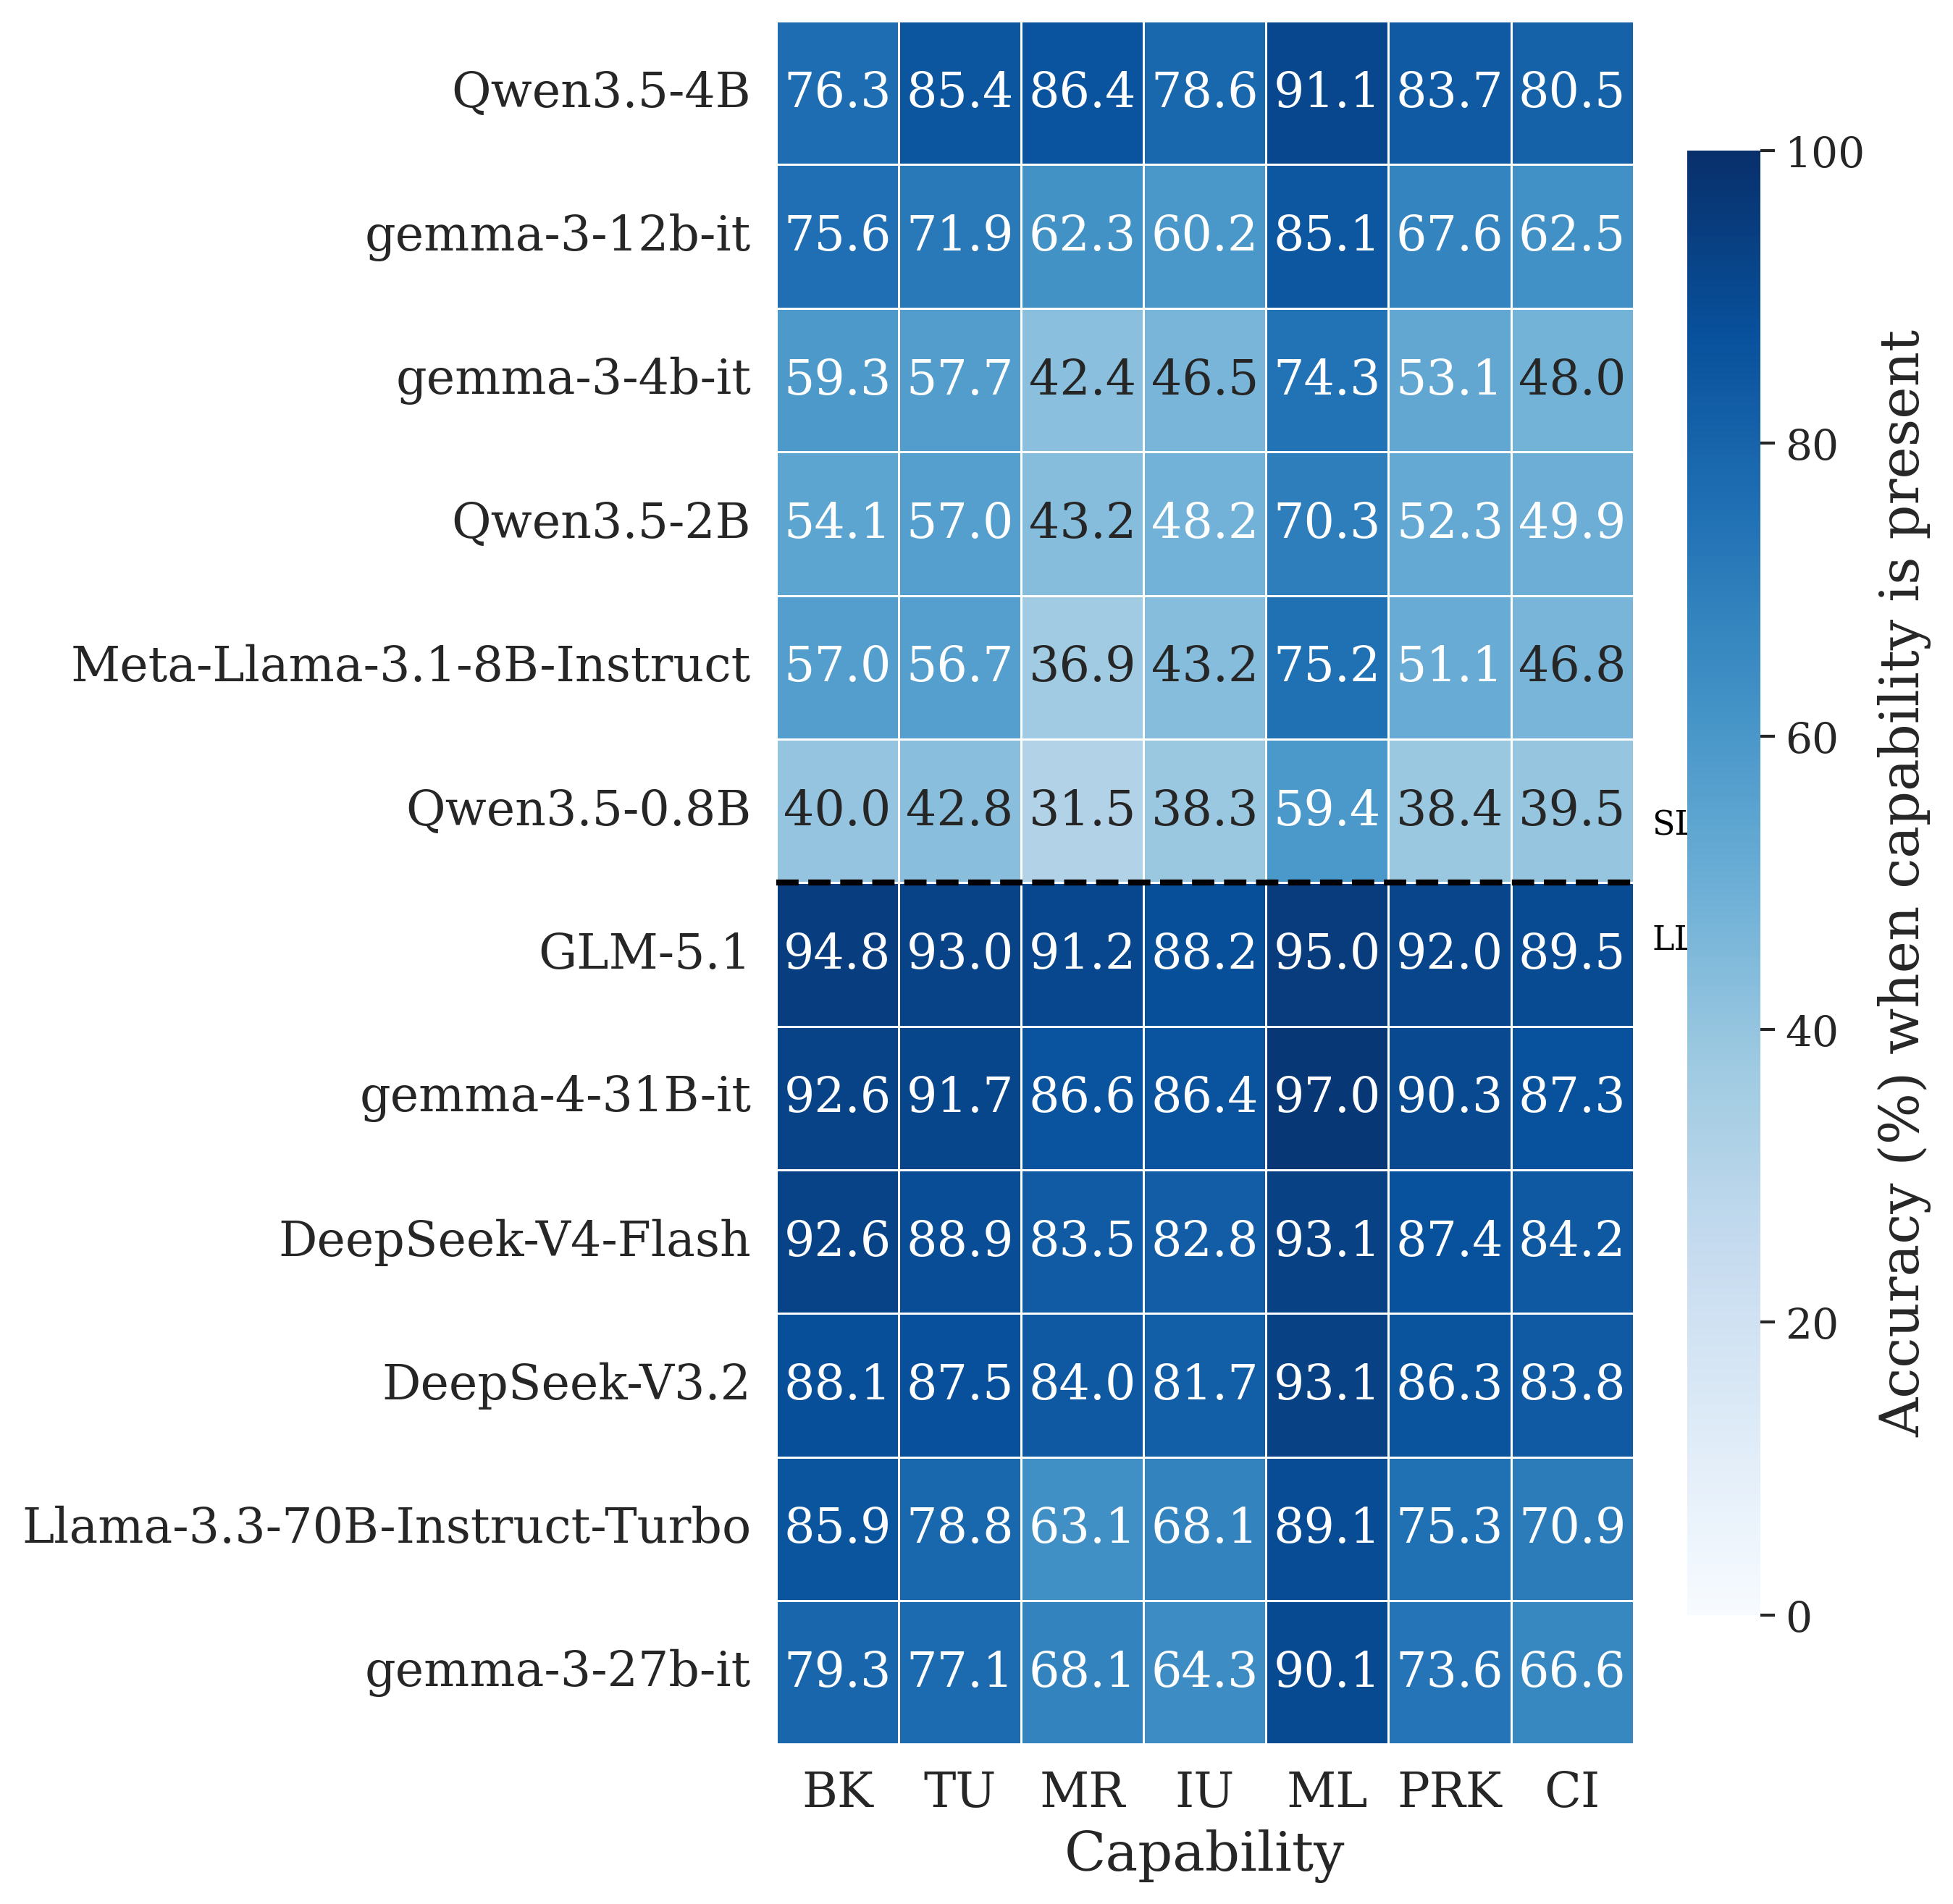
\includegraphics[width=\textwidth]{figures/capability_true_bluex.png}
      \caption{Competencies Present (True)}
    \end{subfigure}%
    \hspace{0.02\textwidth}
    \begin{subfigure}{0.55\textwidth}
      \centering
      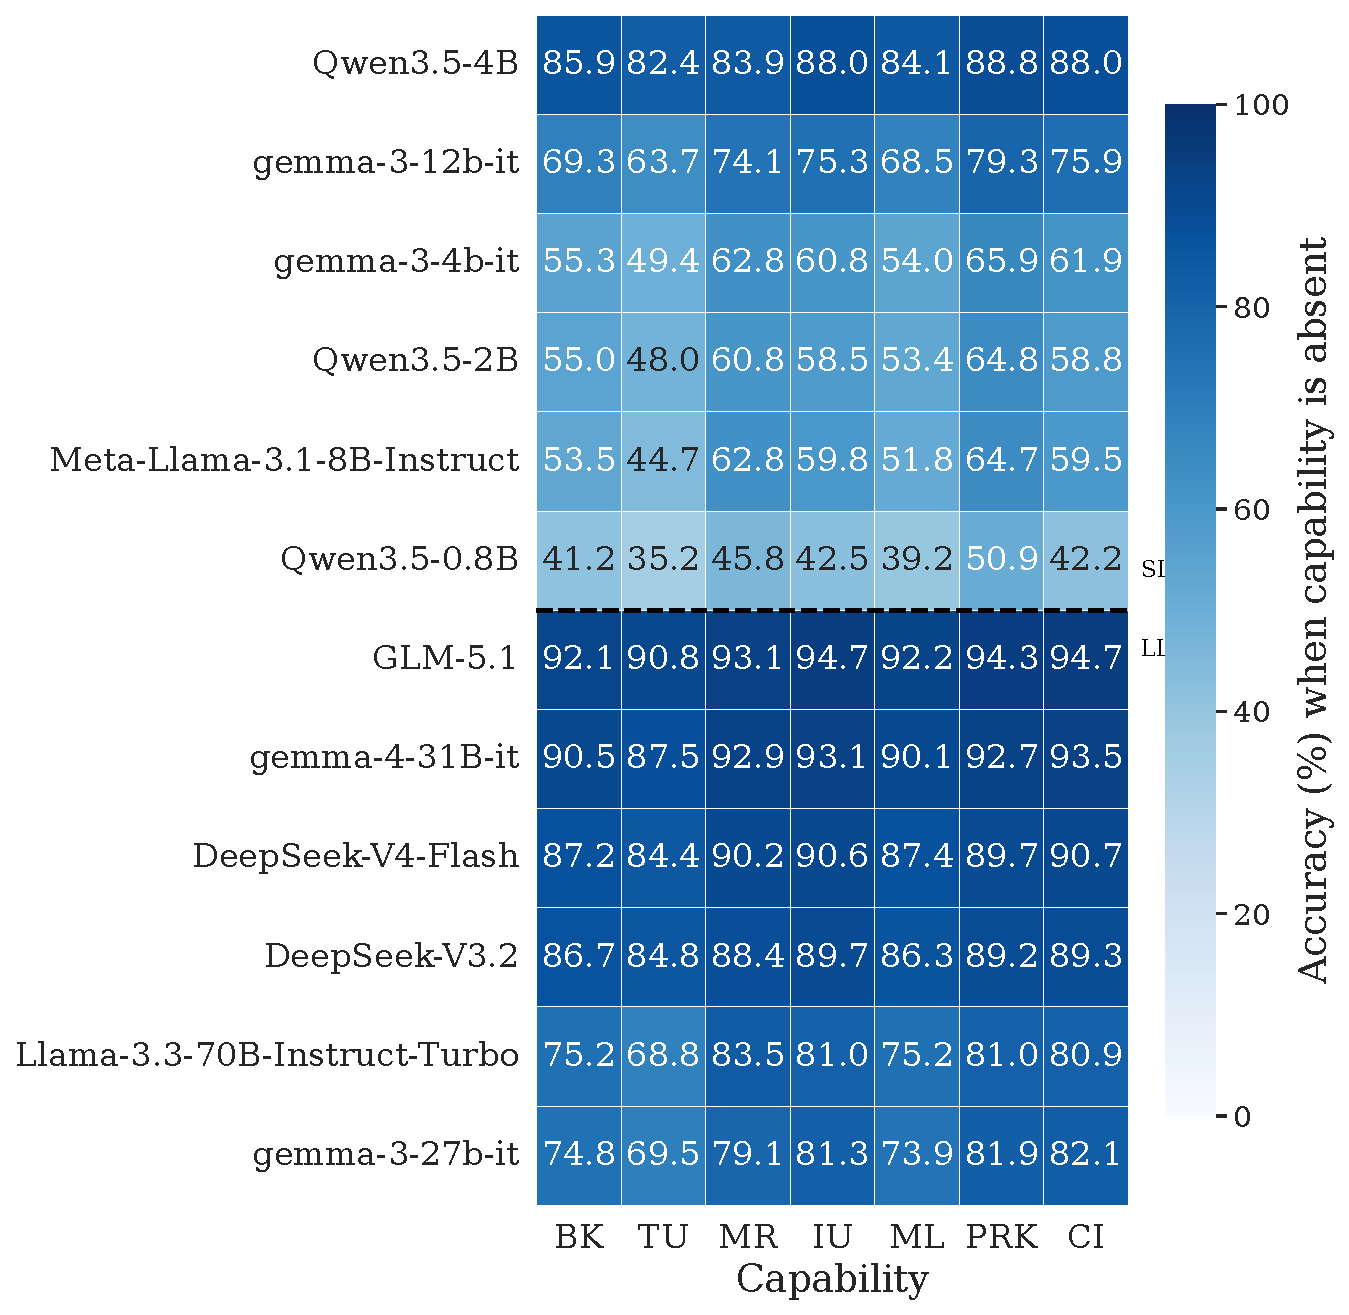
\includegraphics[width=\textwidth]{figures/capability_false_bluex.pdf}
      \caption{Competencies Absent (False)}
    \end{subfigure}%
  }
  \caption{Accuracy heatmaps separating questions by individual BLUEX capability annotations (e.g., MR, CI, TU).}
  \label{fig:bluex_capabilities}
\end{figure}

\subsection{Performance by Modality}
Our modality analysis separates originally text-only questions from questions whose visual content was replaced by Seed-1.8 textual descriptions, allowing us to estimate the remaining penalty associated with visual information when models are evaluated through a text-only interface. As shown in Fig.~\ref{fig:modality_enem} for the ENEM dataset, textual substitution enables all models to process originally visual questions, but smaller models still show a clear performance penalty.

\begin{figure}[htbp]
\centering
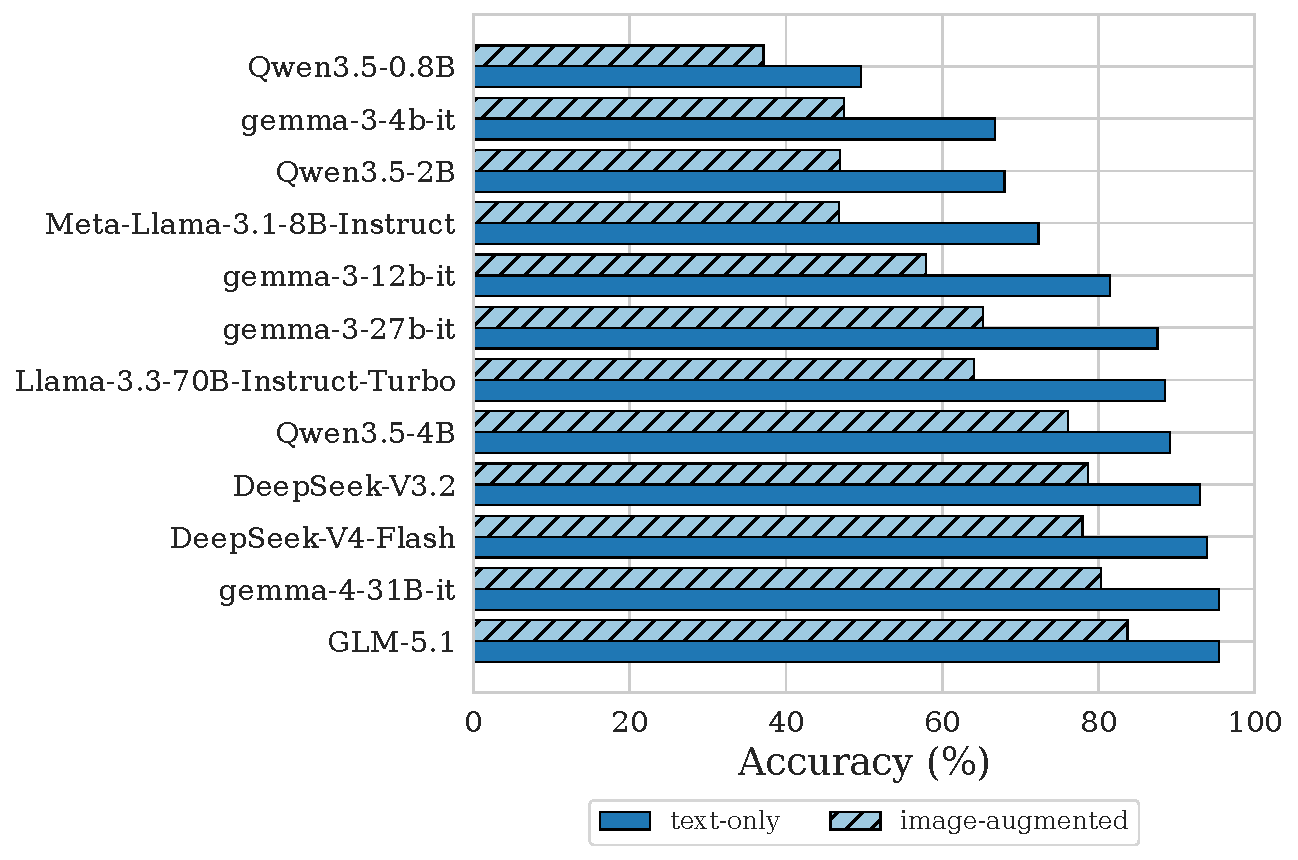
\includegraphics[width=0.85\textwidth]{figures/modality_enem.pdf}
\caption{Comparative accuracy isolating strictly textual queries versus image-augmented targets mapped to VLM descriptions (ENEM dataset).}
\label{fig:modality_enem}
\end{figure}

The results for the case with textual substitution indicate that accuracy generally degrades compared to pure-text problems. Translating complex visual stimuli, such as schematic diagrams or historic art, into text may introduce ambiguity that smaller models are less able to resolve, although this effect would need further verification. Behavior also appeared broadly similar across FUVEST and Unicamp (charts omitted for brevity), which may suggest that visual substitution remains a bottleneck for highly compact NLP pipelines acting autonomously on multimodal downstream tasks.

\subsection{Performance by Testing Year}
Finally, we mapped longitudinal correctness to evaluate model resilience chronologically. Observing Fig.~\ref{fig:testing_year}, models showcase distinct temporal signatures.

\begin{figure}[htbp]
  \centering
  \makebox[\textwidth][c]{%
    \begin{subfigure}{0.55\textwidth}
      \centering
      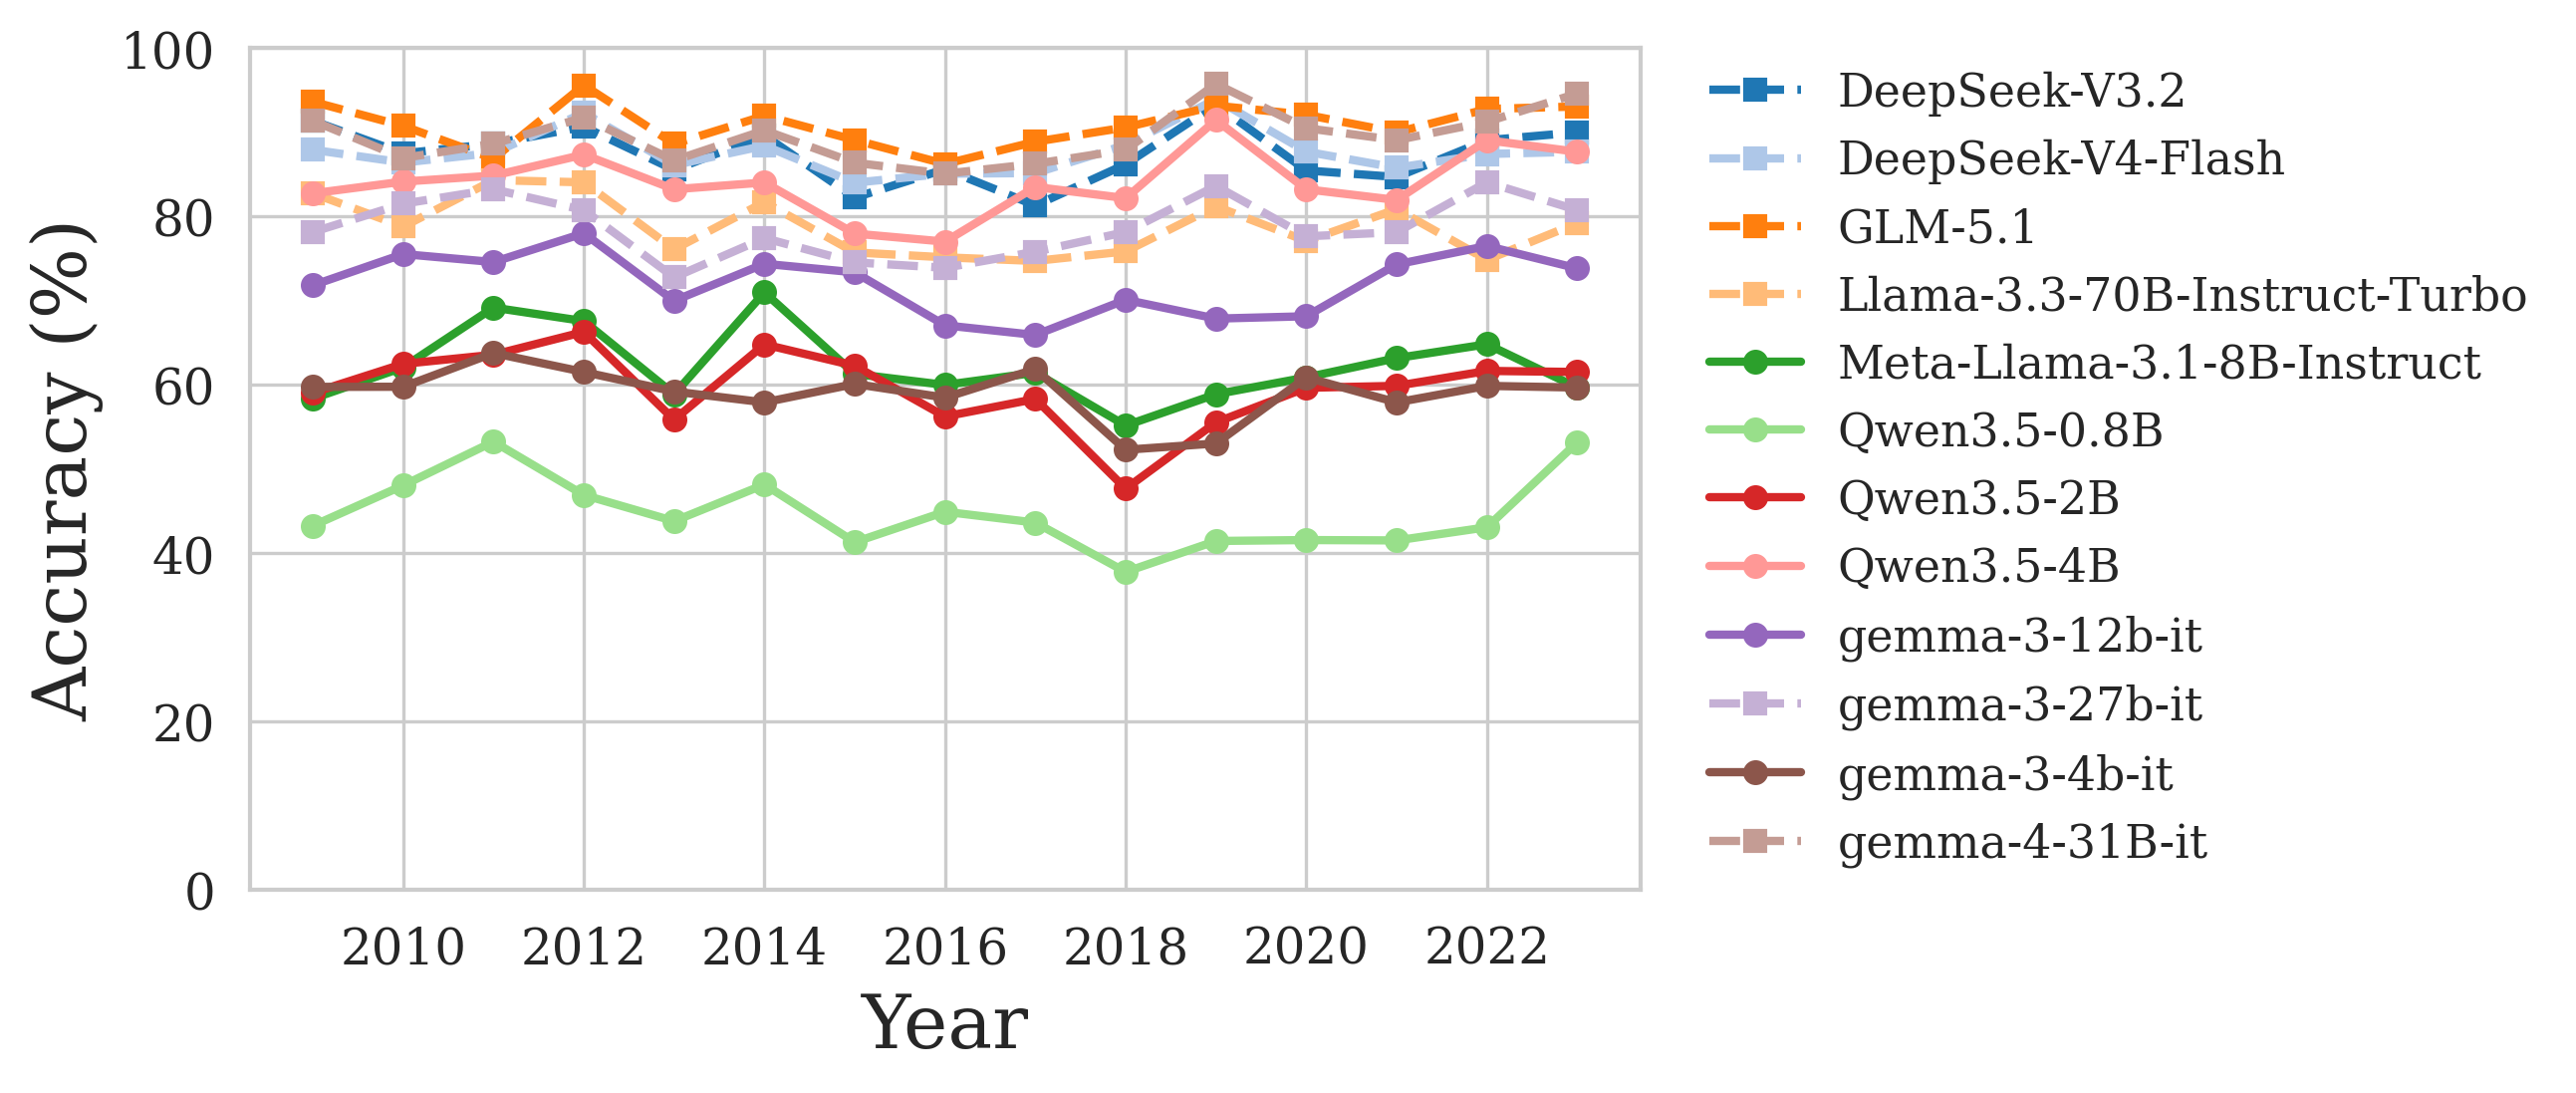
\includegraphics[width=\textwidth]{figures/year_enem.png}
      \caption{ENEM}
    \end{subfigure}%
    \hspace{0.02\textwidth}
    \begin{subfigure}{0.55\textwidth}
      \centering
      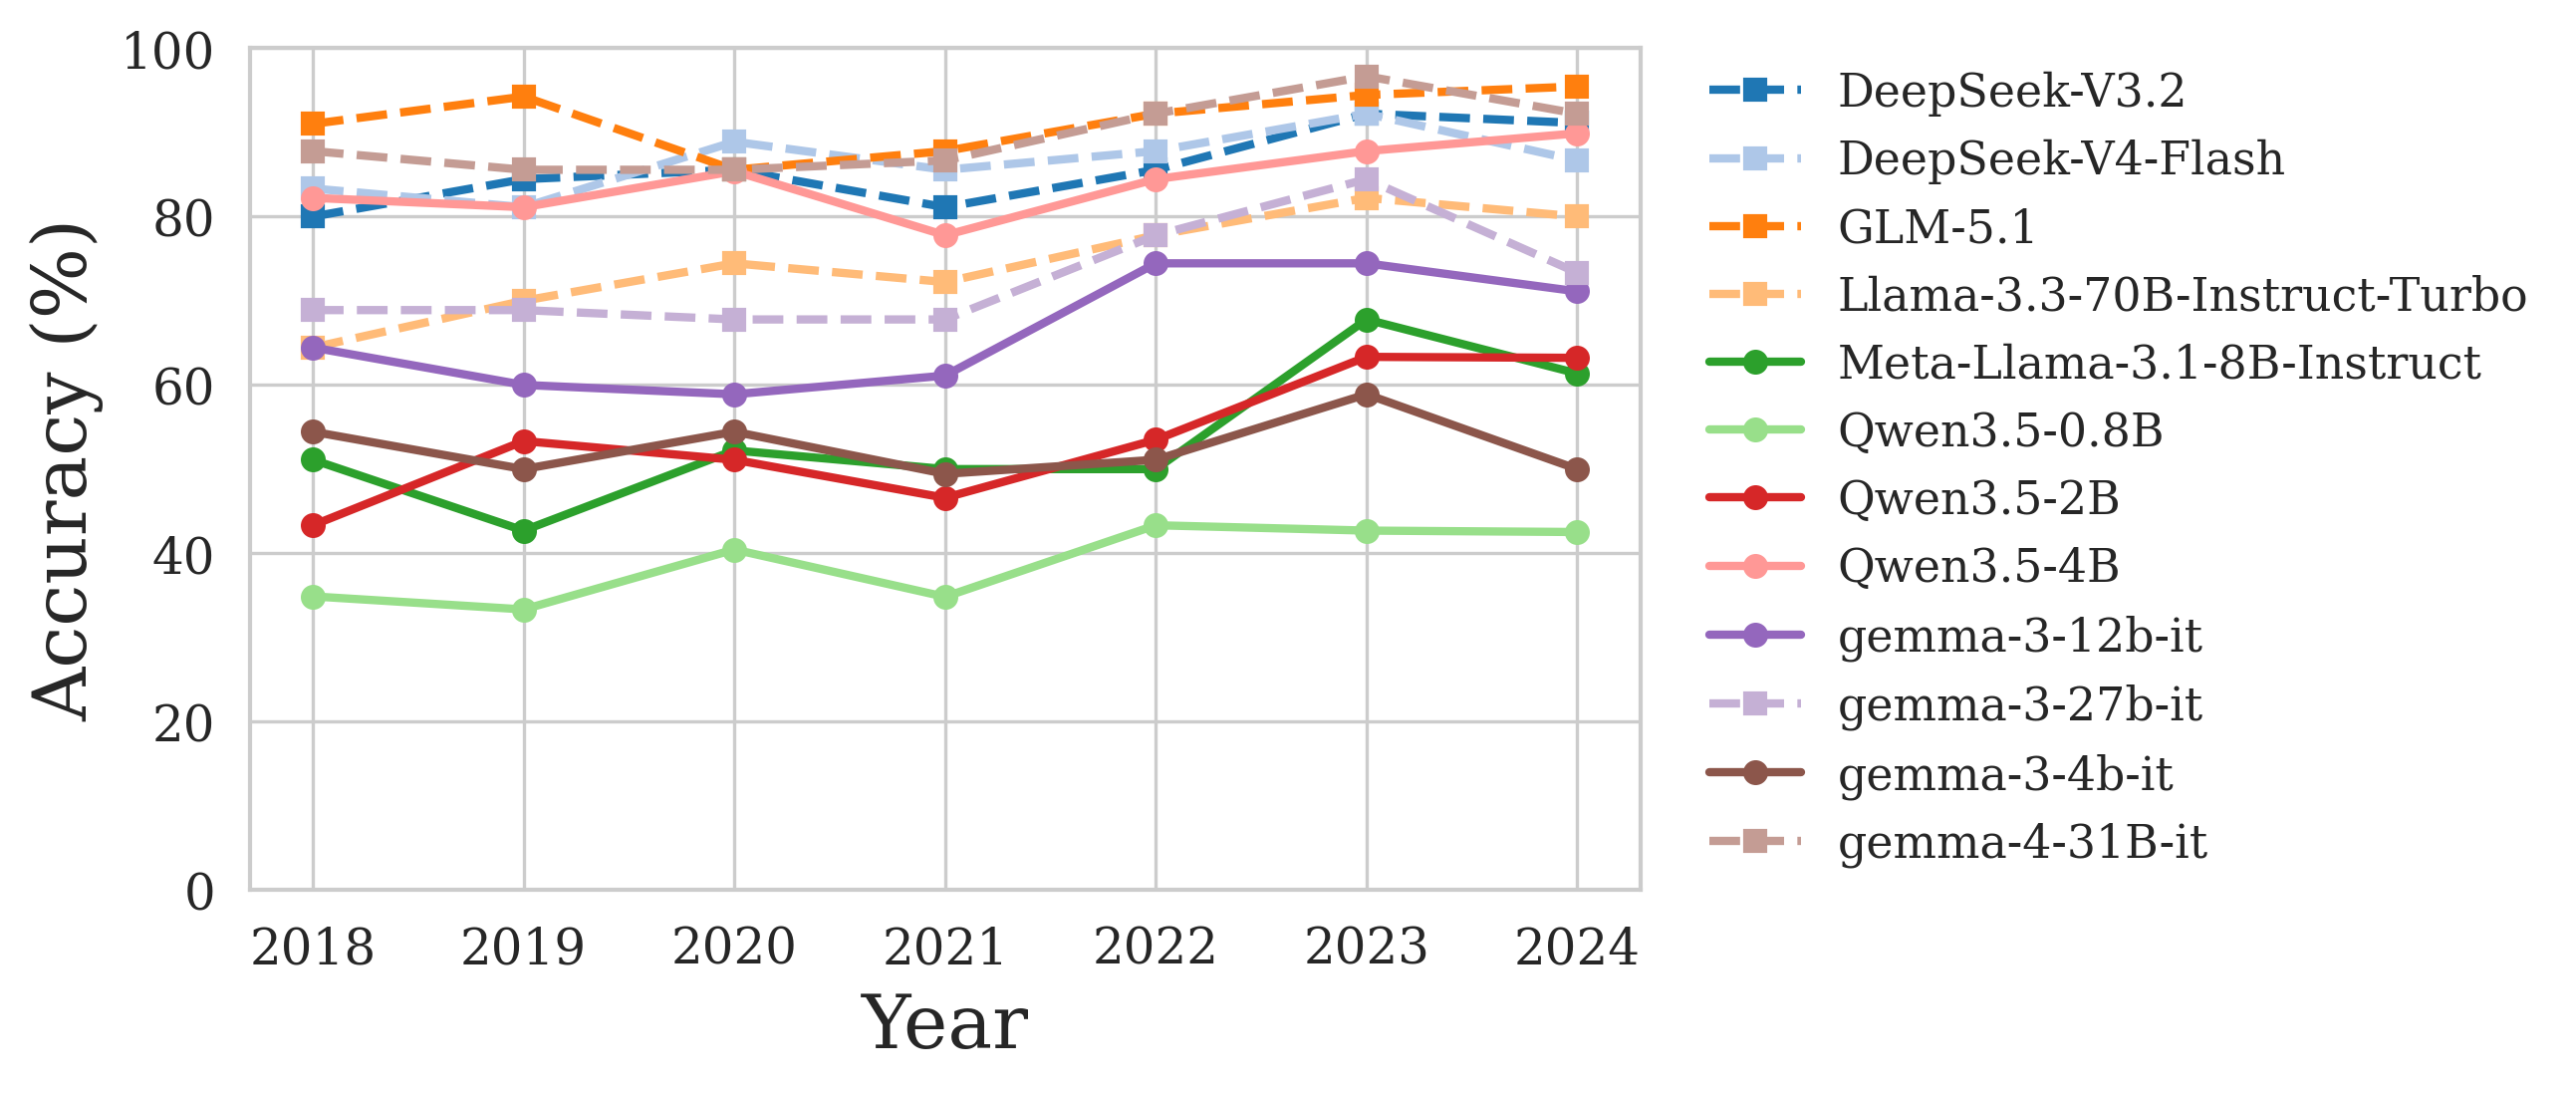
\includegraphics[width=\textwidth]{figures/year_fuvest.png}
      \caption{FUVEST}
    \end{subfigure}%
  }

  \vspace{0.4cm}

  \begin{subfigure}{0.65\textwidth}
    \centering
    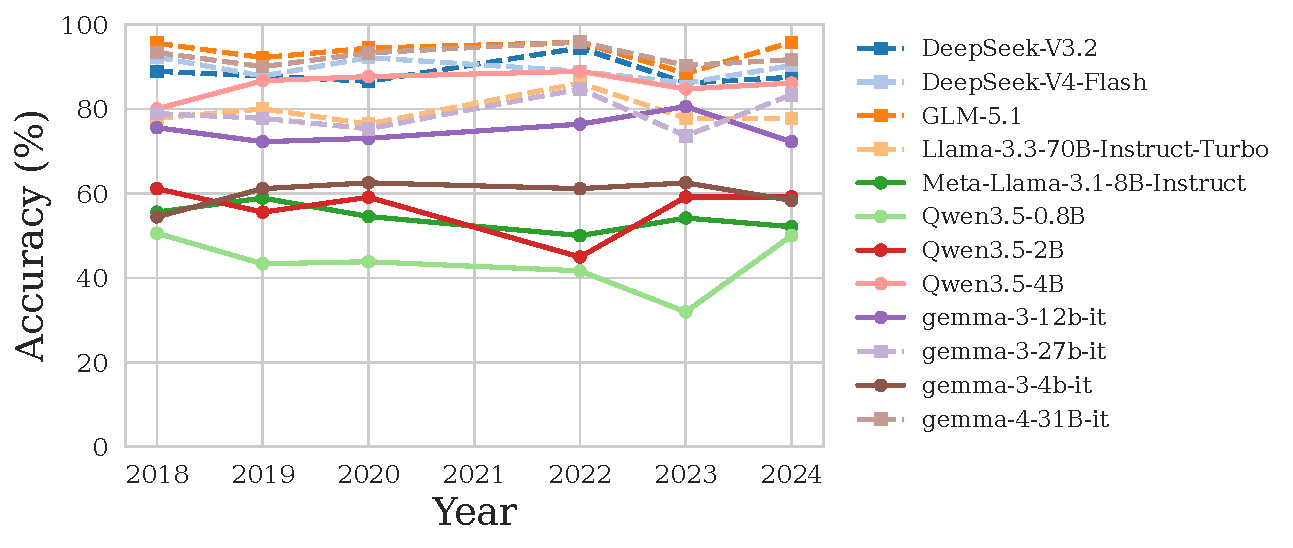
\includegraphics[width=\textwidth]{figures/year_unicamp.pdf}
    \caption{Unicamp}
  \end{subfigure}
  \caption{Longitudinal accuracy tracking per year spanning ENEM, FUVEST, and Unicamp.}
  \label{fig:testing_year}
\end{figure}

Generally, larger reference models maintain stable performance across testing years. SLMs, on the other hand, demonstrated higher volatility. Their accuracy fluctuates more visibly across years, but this pattern should be interpreted cautiously because yearly subsets may differ in size, subject composition, difficulty, and potential training-data exposure. The temporal analysis therefore serves primarily as a robustness diagnostic rather than as evidence of a specific causal factor.

\section{Discussion}
\label{sec:discussion}

In this section, we formalize adherence to the zero-shot protocol, investigate reasoning deviations and failures uniquely prevalent in smaller architectures, and delineate the cost-benefit trade-offs of deploying SLMs against larger frontier variants.

Tracking zero-shot adherence reveals that enforcing structured JSON output remains highly challenging at smaller parameter scales. While larger reference models achieved near-perfect adherence, smaller architectures exhibited distinct instruction-following breakdown modes. These formatting anomalies are evaluated independently from raw accuracy to decouple structural syntax alignment from core thematic correctness.

A critical failure pattern in reasoning-focused architectures (particularly smaller Qwen variants) involves exhausting the generation token budget by emitting overly long intermediate explanations before producing the required \texttt{predicted\_answer} field. Conversely, models like Gemma-3-4B and Llama-3.1-8B successfully avoided these length traps but occasionally triggered minor syntax errors, which our tolerant parser recovered in the majority of instances.

\section{Conclusion}
\label{sec:conclusion}

This paper presents one of the first systematic evaluations of Small Language Models in Brazilian high-stakes educational exams, combining Portuguese reasoning with image-based questions through textual descriptions. This setting fills an important gap left by prior benchmarks, which are often centered on English or on native multimodal models, and offers a practical way to study SLMs under realistic educational conditions. Our results show that, despite their cost efficiency, compact models still struggle with mathematical reasoning, formal inference, and strict output adherence in zero-shot evaluation.

While our benchmark provides a useful overview, it still has important constraints. Replacing native multimodal processing with Seed-1.8 text descriptions removes true spatial reasoning from the SLM evaluation, so failures on multimodal questions may reflect limitations of the descriptions rather than the models themselves. Because we used generic rather than question-aware prompts, some critical visual details may also have been omitted, potentially underestimating performance. Methodologically, relying on a third-party API (DeepInfra) introduced minor non-determinism, preventing bit-exact reproducibility even at temperature zero, and our current zero-shot setting does not capture the gains that multi-shot learning, Chain-of-Thought, or other scaffolding may provide. Finally, comparing dense and MoE architectures makes nominal parameters, active computation, and cost harder to align directly. Future work should validate description strategies with human inputs or calibration sets and test emerging native multimodal SLMs with direct visual inputs.

For future work, we intend to explore targeted fine-tuning strategies to improve mathematical reasoning and format adherence in SLMs. Additionally, we plan to evaluate native multimodal SLMs to directly process visual assets, bypassing the limitations introduced by intermediate textual descriptions, and to investigate few-shot or chain-of-thought methodologies to further close the performance gap with larger models.

\appendix
\section{Prompts}
\label{sec:prompts}

This appendix provides the exact prompts used to evaluate the language models and generate the visual descriptions via Vision-Language Models (VLMs).

\subsection*{Language Model Evaluation Prompts}
To strictly enforce output reasoning and structure without requiring task-specific fine-tuning, models received the following system prompt:

\begin{verbatim}
Você é um assistente especialista em questões de vestibulares e do 
ENEM. Sempre responda em PORTUGUÊS. Leia a questão com atenção e 
escolha uma alternativa. Sua saída DEVE ser um único objeto JSON no 
seguinte formato, sem texto antes nem depois:
{
  "reasoning_summary": "<até 150 palavras>",
  "predicted_answer": "<LETRA_OU_VALOR>"
}
Regras:
- predicted_answer deve ser EXATAMENTE um dos valores permitidos para 
  esta questão (mostrados abaixo).
- reasoning_summary deve ter no máximo 150 palavras, em português, e
  deve explicar como você chegou a sua resposta.
- Não use crases, não use markdown, não envolva o JSON em ``` ou
  similares.
- Se houver descrições de imagens entre [início da descrição da imagem ...]
  e [fim da descrição da imagem ...], trate-as como a imagem real.
\end{verbatim}

The corresponding user prompt injects the context for each individual question:

\begin{verbatim}
# Questão ({dataset}, {year}, {subject})
{question_text}
# Alternativas
{alternatives_block}
# Valores permitidos para predicted_answer
{allowed_values}
Responda APENAS com o JSON.
\end{verbatim}

\subsection*{Multimodal Description Generation Prompt}

For the preliminary step involving the conversion of visual elements into text (utilized by ByteDance Seed-1.8), the models received the payload configured with a simple, direct instructional string accompanying the binary image:
\begin{verbatim}
Descreva a imagem e seus detalhes em português.
\end{verbatim}

\bibliographystyle{apalike}
\bibliography{references}

\end{document}